
\documentclass[15pt,a4paper]{book}

\usepackage{amsmath, amsthm, amssymb} 
\usepackage{graphicx} % For including graphics
\usepackage{hyperref} % For clickable links
\usepackage{bookmark} % Better control over bookmarks
\usepackage{geometry} % Customize page layout
\usepackage{xcolor} % Colors for text and graphics
\usepackage{enumitem} % Customizable lists
\usepackage{fancyhdr} % Header and footer
\usepackage{titlesec} % Custom section/chapter titles
\usepackage[toc,page]{appendix} % For the appendix
\usepackage{longtable} % For tables spanning multiple pages
\usepackage{mathrsfs} % For script fonts in math mode
\usepackage{tocloft} % Custom table of contents
\usepackage{datetime2} % For dates
\usepackage{caption} % For better control over captions
\usepackage{float} % Fine control over figure/table placement
\usepackage{imakeidx} % For index
\usepackage[contents={},placement=page]{background} % For bands
\usepackage{pastel} % For color
\usepackage{etoolbox}

% Custom Theorem Styles
\newtheorem{theorem}{Theorem}[chapter]
\newtheorem{lemma}[theorem]{Lemma}
\newtheorem{proposition}[theorem]{Proposition}
\newtheorem{corollary}[theorem]{Corollary}
\theoremstyle{definition}
\newtheorem{definition}[theorem]{Definition}
\newtheorem{example}[theorem]{Example}
\newtheorem{remark}[theorem]{Remark}

\renewcommand{\cftchapfont}{\normalfont} % Remove bold for chapter names
\renewcommand{\cftchappagefont}{\normalfont} % Remove bold for chapter page numbers
\renewcommand{\qedsymbol}{$\blacksquare$}
% macros.tex
\usepackage{mathtools}
\newcommand{\defeq}{\vcentcolon=}
\newcommand{\eax}[1]{\emph{#1}\index{#1}} % Macro for emphasis and index
\newcommand{\abs}[1]{\left| #1 \right|} % Absolute value
\newcommand{\1}{\textbf{1}}
\newcommand{\N}{\mathbb{N}} % Natural Numbers
\newcommand{\R}{\mathbb{R}} % Real numbers
\newcommand{\Z}{\mathbb{Z}} % Integers
\newcommand{\Q}{\mathbb{Q}} % Rationals
\newcommand{\C}{\mathbb{C}} % Complex numbers
\newcommand{\F}{\mathbb{F}} % Field
\newcommand{\cP}{\mathcal{P}}
\newcommand{\cH}{\mathcal{H}}
\newcommand{\cJ}{\mathcal{J}}
\newcommand{\cR}{\mathcal{R}}
\newcommand{\cB}{\mathcal{B}}
\newcommand{\cC}{\mathcal{C}}
\newcommand{\cI}{\mathcal{I}}
\newcommand{\cD}{\mathcal{D}}
\newcommand{\cF}{\mathcal{F}}
\newcommand{\cZ}{\mathcal{Z}}
\newcommand{\cO}{\mathcal{O}}
\newcommand{\osc}{\text{osc}}
\newcommand{\eps}{\varepsilon}  
\newcommand{\toinf}{\to \infty}
\newcommand{\norm}[1]{\left\lVert#1\right\rVert} % Norm of a vector
\newcommand{\ip}[1]{\langle#1\rangle} % Inner product
\newcommand{\intr}{\operatorname{int}} % Interior of a set
\newcommand{\Bin}{\operatorname{Bin}} % Binomial distribution
\newcommand{\Ber}{\operatorname{Ber}} % Bernoulli distribution
\newcommand{\Poi}{\operatorname{Poisson}} % Poisson distribution


% Custom Notation List Environment
\newlist{notationlist}{description}{1}
\setlist[notationlist]{font=\bfseries,labelsep=1em}

% Geometry Settings
\geometry{
    top=2.5cm,
    bottom=2.5cm,
    left=2.5cm,
    right=2.5cm,
}

% Hyperref Colors
\hypersetup{
    colorlinks=true,
    linkcolor=black,
    urlcolor=cyan,
    citecolor=red
}

\renewcommand{\chaptermark}[1]{\markboth{#1}{}}
\renewcommand{\sectionmark}[1]{\markright{#1}}

% Custom Headers
\pagestyle{fancy}
\fancyhf{}
\fancyhead[L]{\leftmark} % Chapter name on top left
\fancyhead[R]{\rightmark}  % section name on top right
\fancyfoot[C]{\thepage}

\renewcommand{\headrulewidth}{0pt}
\renewcommand{\footrulewidth}{0pt}

% Making index
\makeindex[intoc]

% Title Formatting
\titleformat{\chapter}[display]
  {\normalfont\Large\bfseries \centering}
  {\chaptername\ \thechapter}{20pt}{\Huge \centering}

\titlespacing*{\chapter}{0pt}{20pt}{100pt}

% === Colored header/footer bands ===
\backgroundsetup{
  scale=1,
  angle=0,
  opacity=1,
  contents={
    % Top band
    \begin{tikzpicture}[remember picture,overlay]
      \fill[\subjectcolor!40!white]
        (current page.north west) rectangle ([yshift=-2.2cm]current page.north east);
    \end{tikzpicture}
    % Bottom band
    \begin{tikzpicture}[remember picture,overlay]
      \fill[\subjectcolor!40!white]
        ([yshift=2.1cm]current page.south west) rectangle (current page.south east);
    \end{tikzpicture}
  }
}

\begin{document}

\pagestyle{empty}

\begin{titlepage}
    \begin{tikzpicture}[remember picture, overlay]
        \fill[\subjectcolor!60!white] 
            (current page.south west) rectangle (current page.north east);
    \end{tikzpicture}

    \begin{center}
        \vspace*{\fill}
        {\Huge\bfseries\color{black!90} \MakeUppercase{Introduction to Statistical Inference}\par}
        \vspace{0.5cm}
        {\Large\color{black!90} Sangita Das, notes by Ramdas Singh\par}
        \vspace{0.5cm}
        {\large\color{black!90} Third Semester\par}
        \vspace*{\fill}
    \end{center}
\end{titlepage}

\clearpage

\pagenumbering{roman}

\chapter*{List of Symbols}
\begin{notationlist}
    \item Placeholder
\end{notationlist}

\newpage
\setcounter{tocdepth}{2}
\tableofcontents

\newpage
\pagenumbering{arabic}
\pagestyle{fancy}


% Include chapters below
\chapter{INTRODUCTION TO GROUP THEORY}

\section{Set Theory}
\textit{July 22nd.}

We begin with some basic assumptions to introduce set theory. The symbol $\in$ is used to denote membership in a set. A statement using this in set theory may be stated as $x \in y$, which can be either true or false. Once we have developed this language to discuss sets, we can introduce some axioms.
\begin{axiom}
    There exists a set with no elements, the \eax{empty set} $\emptyset$.
\end{axiom}
Formally, the above axiom is $\exists x (\forall y (y \notin x))$.
\begin{axiom}
    Two sets are equal if they have the same elements.
\end{axiom}
From the above two axioms, we can infer a unique empty set. A notion of subsets may also be declared.
\begin{definition}
    We say the set $A$ is a \eax{subset} of the set $B$, denoted $A \subseteq B$, if every element of $A$ is also an element of $B$.
\end{definition}
We also have a bunch of similarity axioms stated below.
\begin{axiom}[Similarity axioms]
    We have the following:
    \begin{enumerate}
        \item If $x, y$ are sets, then $\{x, y\} \Rightarrow \{x, \{x, y\}\}$ (not an ordered pair).
        \item If $A$ is a set, then $\bigcup A = \{x \mid \exists y \in A,\ x \in y\}$ is a set.
        \item There exists a \eax{power set} for every set; given a set $A$, there exists a set $P(A)$ such that for all $B \subseteq A$, $B \in P(A)$. Formally, $\forall A \exists P(A) (\forall B \subseteq A, B \in P(A))$.
        \item The \eax{infinite axiom}: Formally, $\exists I (\emptyset \in I \wedge \forall y \in I (P(y) \in I))$.
        \item If $A$ and $B$ are sets, then $A \times B = \{(x,y) \mid x \in A, y \in B\}$ is a set.
    \end{enumerate}
\end{axiom}
Before discussing the last axiom, we define a relation on sets.
\begin{definition}
    A \eax{relation} $R$ on a set $A$ is a subset $R \subseteq A \times A$. If $(x,y) \in R$, we write $xRy$.
\end{definition}
\begin{axiom}[The \eax{axiom of choice}]
    Let $A$ be a collection of non-empty and disjoint sets. Then there exists a set $C$ consisting of exactly one element from each set in $A$.
\end{axiom}


\begin{definition}
    A relation $R$ on a set $A$ is said to be:
    \begin{itemize}
        \item \eax{reflexive} if $xRx \forall x \in A$,
        \item \eax{symmetric} if $xRy \Rightarrow yRx$,
        \item \eax{transitive} if $xRy \wedge yRz \Rightarrow xRz$,
        \item \eax{antisymmetric} if $xRy \wedge yRx \Rightarrow x = y$.
    \end{itemize}
\end{definition}

\begin{definition}
    A \eax{partial order} on a set $A$ is a reflexive, transitive, and antisymmetric relation on $A$.
\end{definition}
Some examples of partially ordered sets include $(R, \leq)$, $(P(\R), \subseteq)$.

\begin{definition}
    A \eax{total order} $R$ on a set $A$ is a partial order such that for all $x,y \in A$, either $xRy$ or $yRx$.
\end{definition}
Again, $(R, \leq)$ is a totally ordered set, but not $(P(\R), \subseteq)$.
\begin{definition}
    A total order $\leq$ on a set $A$ is said to be a \eax{well-order} if given any non-empty subset $B \subseteq A$, there exists $x \in B$ such that for all $y \in B$, $x \leq y$.
\end{definition}

The below theorem may be derived from the above definitions and axioms.

\begin{theorem}[The \eax{well-ordering principle}]
    Every set can be well-ordered.
\end{theorem}
We may note that the well-ordering principle and the axiom of choice are equivalent.

\begin{definition}
    A \eax{chain} in partially ordered set $A$, with relation $\prec$, is a subset of $A$ which is totally ordered with respect to $\prec$.
\end{definition}
\begin{definition}
    Let $C \subseteq A$ be a subset in a partially ordered set $(A, \prec)$. An element $x \in A$ is an upper bound of $C$ if for all $y \in C$, $y \prec x$.
\end{definition}
\begin{definition}
    An element $x \in A$ is a \eax{maximal element} of a partially ordered set $(A, \prec)$ if for all $y \in A$, $x \prec y \Rightarrow x = y$.
\end{definition}
\begin{lemma}[\eax{Zorn's lemma}]
    Let $A$ be a set and let $\prec$ be a partial order on $A$ such that every chain in $A$ has an upper bound. Then $A$ has a maximal element.
\end{lemma}

\begin{theorem}
    The following are equialent:
    \begin{enumerate}
        \item The axiom of choice,
        \item The well-ordering principle,
        \item Zorn's lemma.
    \end{enumerate}
\end{theorem}

\begin{definition}
    A relation $R$ on a set $A$ is said to be an \eax{equivalence relation} if it is reflexive, symmetric, and transitive. Let $x \in A$. Then $[x] = \{yRx \mid y \in A\} \subseteq A$ is called the \eax{equivalence class} of $x$.
\end{definition}

We note that $\bigcup_{x \in A} [x] = A$ and for $x,y \in A$, either $[x] \cap [y] = \emptyset$ or $[x] = [y]$. Thus, we get a partition of $A$ into equivalence classes.

Let $I$ be an indexing set, and let $A_{i}$ be sets for all $i \in I$. Then the existence of $\text{X}_{i \in I} A_{i} = \{f:I \to \overset{\cdot}{\bigsqcup} A_{i} \mid f(i) \in A_{i} \text{ for all } i \in I\}$ is another way of stating the axiom of choice.

\begin{theorem}[The \eax{principle of induction}]
    Let $S(n)$ be statements about the naturals $n \in \N$. Suppose $S(1)$ holds and for all $k \in \N$, $S(k) \Rightarrow S(k+1)$. Then $S(n)$ holds true for all $n \in \N$.
\end{theorem}

Let $I$ be a well-ordered set and let $S(i)$ be statements for all $i \in I$. Suppose that if $S(j)$ holds for all $j < i$, then $S(i)$ holds. Then $S(i)$ holds for all $i \in I$. This is the \eax{principle of transfinite induction}, which is also equivalent to the axiom of choice. We now properly introduce the theory of groups.

\section{Groups}
We first define a group.
\begin{definition}
    A \eax{group} is a triple $(G, \cdot, e)$ where $G$ is a set, $\cdot: G \times G \to G$ is a binary operation on $G$, and $e \in G$ is an element of $G$ satisfying the following axioms:
    \begin{itemize}
        \item The property of \eax{associativity}: For $a,b,c \in G$, $(a \cdot b) \cdot c = a \cdot (b \cdot c)$.
        \item The property of the \eax{identity element}: For all $a \in G$, $a \cdot e = e \cdot a = a$. $e$ is referred to as the identity element.
        \item The existence and property of the \eax{inverse element}: For all $a \in G$, there exists $b \in G$ such that $a \cdot b = b \cdot a = e$. $b$ is referred to as the inverse of $a$ and is denoted by $a^{-1}$.
    \end{itemize}
    In addition, $(G,\cdot,e)$ is also termed an \eax{abelian group} if for all $a,b \in G$, $a \cdot b = b \cdot a$, that is, commutativity holds.
\end{definition}
Some examples include $(\Z, +), (\Q, +), (\R, +), (\C, +)$. The set $(\Q, \cdot)$ is not a group since $0$ does not have an inverse. However, $(\Q^{\ast}, \cdot)$ is a group, where $\Q^{\ast} = \Q\setminus\{0\}$. All these groups are also abelian. An example of a non-abelian group is $S_{n}$, the set of all bijections from $\{1,2,\ldots,n\}$ to itself, under the binary operation of composition of functions. Another non-abelian group is $(GL_{n}(\R), \cdot)$, for $n \geq 2$, the set of all invertible real matrices.
\chapter{POINT ESTIMATION}

We begin with a definition.

\begin{definition}
    A \eax{point estimator} is a function $W$ of the sample, mapping into the parameter space $\Theta$ of the parameter $\theta$ of interest. The value $W(X)$ is called a \eax{point estimate} of $\theta$.
\end{definition}

Various methods of point estimation are discussed in this chapter, including the method of moments, maximum likelihood estimation, and Bayes estimation.

\section{Estimators}
\subsection{Method of Moments}
Let $X_{1},\ldots,X_{n}$ be a sample from a population with a probability distribution function and probability density function. The \eax{method of moments} estimators are found by equating the first $k$ sample moments to the corresponding $k$ population moments and solving the resulting system of simultaneous equations. Here, the $k^{\text{th}}$ sample moment and the $k^{\text{th}}$ population moment are given as
\begin{align}
    m_{k} = \frac{1}{n} \sum_{j=1}^{n} X_{j}^{k} \qquad \text{and} \qquad \mu_{k}' = E[X^{k}]
\end{align}
respectively. For $\mu_{j}' = \mu_{j}'(\theta_{1},\ldots,\theta_{i})$, with $1 \leq j \leq k$, the estimators are obtained by solving the equations
\begin{align}
    m_{j} = \mu_{j}'(\theta_{1},\ldots,\theta_{i}) \qquad \text{for } 1 \leq j \leq k.
\end{align}

\subsection{Maximum Likelihood Estimators}

Let $X_{1},\ldots,X_{n}$ be an independent and identically distributed sample from a population with a probability distribution/mass function $f(\underline{x} \mid \theta_{1},\ldots,\theta_{k})$. The \eax{likelihood function} is defin as
\begin{align}
    L(\underline{\theta} \mid \underline{x}) = L(\theta_{1},\ldots,\theta_{k} \mid x_{1},\ldots,x_{n}) \defeq \prod_{j=1}^{n} f(x_{j} \mid \theta_{1},\ldots,\theta_{k}).
\end{align}

\begin{definition}
    For each sample points, let $\overline{\theta}(\underline{x})$ be a parameter value at which $L(\underline{\theta} \mid \underline{x})$ attains its maxima as a function of $\underline{\theta}$, with $\underline{x}$ held fixed. A \eax{maximum likelihood estimator} (MLE) of the parameter $\theta$ based on a sample $\underline{X}$ is $\hat{\theta}(\underline{X})$.
\end{definition}

\begin{remark}
    \begin{enumerate}
        \item By its contraction, the ranges of the MLE concludes with the range of the parameter.
        \item The MLE is the parameter points for which the observation sample is most likely.
    \end{enumerate}
\end{remark}

If the likelihood function is differentiable in $\theta_{i}$, then possible candidates for the MLE are the values of $(\theta_{1},\ldots,\theta_{k})$ that solve $\frac{\partial}{\partial \theta_{i}}L(\underline{\theta} \mid \underline{x}) = 0$ for $1 \leq i \leq k$. Moreover, we must have $\frac{\partial^{2}}{\partial^{2}\theta_{i}}L(\underline{\theta} \mid \underline{x}) < 0$ for the solution to be a maximum.

\begin{remark}
    \begin{enumerate}
        \item The solutions to the above equation are the only possible candidates for the MLE since the first derivative being zero is only a necessary condition for the maximum and not sufficient.
        \item The zeroes of the first derivatives only locate extreme points in the interior of the domain of the function.
        \item If the extrema occurs on te boundary of the domain, then the first derivative may not be zero. Thus the boundary must be checked separately.
        \item The points where the first derivatives are zero may be local/global maxima or minima. 
    \end{enumerate}
\end{remark}


\begin{example}
    Let us take the example of the binomial distribution, $X \sim \Bin (n,p)$. The likelihood function is given by $L(p \mid x) = \binom{n}{x} p^{x} (1-p)^{n-x}$, where $0 < p < 1$. We have
    \begin{align}
        \frac{\partial}{\partial p} L(p \mid x) = \frac{dL}{dp}(p \mid x) = 0.
    \end{align}
    This derivative is hard to compute directly. So we take the logarithm (an increasing function) of the likelihood function, and then differentiate.
    \begin{align}
        \implies \frac{d}{dp} \log L(p \mid x) = \frac{x}{p} - \frac{n-x}{1-p} = 0.
    \end{align}
    This gives us $p = \frac{x}{n}$, with the second derivative less than zero, confirming that this is a maximum. Thus, the MLE of $p$ is $\hat{p} = \frac{X}{n}$.
\end{example}

The method in this example is known as \eax{log likelihood estimation}. It is often easier to work with the log likelihood function, especially when dealing with products.

\begin{remark}
    \begin{enumerate}
        \item The MLE may not exist at all or may not be unique.
        \item If $\hat{\theta}$ is the MLE of $\theta$, then $\rho(\hat{\theta})$ is the MLE of $\rho(\theta)$ for any function $\rho$.
    \end{enumerate}
\end{remark}

The following is a vital and important result.
\begin{theorem}
    The MLE depends on $\underline{x}$ only through the sufficient statistic $T(\underline{x})$.
\end{theorem}
\begin{proof}
    We have $L(\theta \mid \underline{x}) = f(\underline{x} \mid \theta) = g(T(\underline{x}),\theta) h(\underline{x})$. Therefore, we have
    \begin{align}
        L(\hat{\theta}(\underline{x}) \mid \underline{x}) = \max_{\theta} g(T(\underline{x}),\theta) h(\underline{x}).
    \end{align}
    Since $h(\underline{x}) > 0$, and does not depend on $\theta$, we must have
    \begin{align}
        L(\hat{\theta}(\underline{x}) \mid \underline{x}) = h(\underline{x}) \max_{\theta} g(T(\underline{x}),\theta)
    \end{align}
    where the maximization is on the part that involves $\underline{x}$ through $T(\underline{x})$ only.
\end{proof}

\subsection{One Parameter Exponential Family in Natural Form}
Recall that the usual density form of the exponential family was given as
\begin{align}
    f(x \mid \theta) = \exp(c(\theta)T(x) + d(\theta) + s(x))\1_{A}(x).
\end{align}
Define $\eta = c(\theta)$ for $\theta \in \Theta$, and let $\Gamma = \{\eta \mid \eta = c(\theta), \theta \in \Theta\}$. We then have
\begin{align}
    f^{\ast}(x \mid \eta) = \exp(\eta T(x) + d_{0}(\eta) + s(x))\1_{A}(x)
\end{align}
where $d_{0}(\eta) = d(c^{-1}(\eta))$ if $c$ is one-one. Moreover,
\begin{align}
    1 &= \int_{A}f^{\ast}(x \mid \eta)dx = \int_{A} \exp(\eta T(x) + d_{0}(\eta) + s(x))dx = \exp(d_{0}(\eta)) \int_{A} \exp(\eta T(x)+s(x))dx \\
    \implies d_{0}(\eta) &= -\log\left( \int_{A} \exp(\eta T(x) + s(x))dx\right). 
\end{align}

\begin{theorem}
    If $X$ has density of the form $f(x \mid \eta) = \exp(\eta T(x) + d_{0}(\eta) + s(x))\1_{A}(x)$ and $\eta$ is an interior points of $H \defeq \{\eta \mid \abs{d_{0}(\eta)} < \infty\}$, then the moment generating function of $T(X)$ exists and is given by
    \begin{align}
        \varphi(s) = E[\exp(sT(X))].
    \end{align}
    Also,
    \begin{align}
        E[T(X)] = -\frac{d}{d\eta} d_{0}(\eta), \qquad \text{ and } \qquad \Var(T(X)) = -\frac{d^{2}}{d\eta^{2}} d_{0}(\eta).
    \end{align}
\end{theorem}

\begin{theorem}
    Let $\{P_{\theta} \mid \theta \in \Theta\}$ be a one parameter exponential family with density $f(x \mid \theta) = \exp(c(\theta)T(x) + d(\theta) + s(x))\1_{A}(x)$ and let $c$ be the interior of $C = \{c(\theta) \mid \theta \in \Theta\}$. Also suppose $\theta \mapsto c(\theta)$ is one-one. If the equation
    \begin{align}
        E_{\theta}[T(X)] = T(x)
    \end{align}
    has a solution $\hat{\theta}(x)$ for which $c(\hat{\theta}(x)) \in C$, then $\hat{\theta}(x)$ is the unique MLE of $\theta$.
\end{theorem}
\begin{proof}
    Since $\theta \mapsto c(\theta)$ is one-one, maximizing the likelihood over $\theta$ is maximizing over $\eta = c(\theta)$. Hence, consider the natural parametrization
    \begin{align}
        f(x \mid \eta) = \exp(\eta T(x) + d_{0}(\eta) + s(x))\1_{A}(x) \text{ for } \eta \in H.
    \end{align}
    $L(\eta \mid x) = \eta T(x) + d_{0}(\eta) + s(x)$, if $x \in A$, is the log likelihood function. Also,
    \begin{align}
        \frac{\partial}{\partial \eta} L(\eta \mid x) = T(x) + d_{0}'(\eta) \text{ and } \frac{\partial^{2}}{\partial \eta^{2}} L(n \mid x) = d_{0}''(\eta).
    \end{align}
    Therefore, we get $\frac{\partial}{\partial \eta} L(\eta \mid x) = T(x) - E_{\eta}[T(x)] = 0$ implying that $E_{\eta}[T(X)] = T(x)$. Now, $\frac{\partial^{2}}{\partial \eta^{2}} L(\eta \mid x) < 0$ so that $L$ is strictly concave. Then we get a unique maxima at $\hat{\eta}(x)$ for which $E_{\eta}[T(X)]_{\eta = \hat{\eta}(x)} = T(x)$.
\end{proof}
\chapter{GRAPHS}


\section{Introduction}
A \eax{graph} is a pair $G = (V,E)$, where $V$ is a set whose elements are called \eax{vertices} and $E \subseteq V \times V$ is a set of unordered pairs $\{v_{1},v_{2}\}$ of vertices, whose elements are called edges. Here, $(v_{1},v_{2})$ and $(v_{2},v_{1})$ are undistinguishable, and are simply denoted by $\{v_{1},v_{2}\}$ or $v_{1}v_{2}$.
\begin{figure}[h]
    \centering
    \begin{tikzpicture}[scale=1,
        every node/.style={circle, draw=\subjectcolor!80!black, fill=\subjectcolor!40!white, inner sep=2pt}]
        % Vertices
        \node (A) at (0, 0.2) {A};
        \node (B) at (2.1, -0.1) {B};
        \node (C) at (1.2, 1.6) {C};
        \node (D) at (3.1, 1.4) {D};
        \node (E) at (4.2, 0.1) {E};

        % Edges
        \draw (A) -- (B);
        \draw (B) -- (C);
        \draw (C) -- (A);
        \draw (B) -- (D);
        \draw (D) -- (E);
    \end{tikzpicture}
\end{figure}

The above shows a simple undirected graph on five vertices $V=\{A,B,C,D,E\}$ with edges $E=\{AB,AC,BC,BD,DE\}$. Here, simple and undirected are also terms to be defined in the context of graph theory.

\begin{definition}
    A graph is called a \eax{simple graph} if it has no loops (edges connecting a vertex to itself) and no multiple edges (more than one edge connecting the same pair of vertices). Otherwise, it is termed a \eax{multigraph}. A graph is called an \eax{undirected graph} if its edges have no orientation; that is, the edge $uv$ is identical to the edge $vu$. Otherwise, it is termed a \eax{directed graph}.
\end{definition}

In directed graphs, or \eax{digraph}s, one deals with $G = (V,E,s,t)$, where $s:E \to V$ gives the \eax{source node} of an edge and $t:E \to V$ gives the \eax{target node} of an edge. In this edge set $E$, $uv \neq vu$, unlike the case of a simple graph.

Structure-preserving maps are useful in graph theory too.

\begin{definition}
    Suppose we have two graphs $G = (V(G),E(G))$ and $H = (V(H),E(H))$. A function $f:V(G) \to V(H)$ is said to be a \eax{graph homomorphism} if $f$ preserves adjacency; that is, if $v_{1}v_{2} \in E(G)$, then $f(v_{1})f(v_{2}) \in E(H)$. If $f$ is also bijective and $f$ and $f^{-1}$ are both graph homomorphisms, then $f$ is termed a \eax{graph isomorphism}.
\end{definition}

We also term the group $\Aut(G)$ as the group of all graph isomorphisms of $G$, with the group operation of composition.

\begin{definition}
    Suppose we have two digraphs $G_{1} = (V_{1},E_{1},s_{1},t_{1})$ and $G_{2} = (V_{2},E_{2},s_{2},t_{2})$. A \eax{digraph homomorphism} is two maps $f_{V}:V_{1} \to V_{2}$ and $f_{E}:E_{1} \to E_{2}$ such that
    \begin{align}
        s_{2}(f_{E}(e)) = f_{V}(s_{1}(e)) \quad \text{ and } \quad t_{2}(f_{E}(e)) = f_{V}(t_{1}(e)).
    \end{align}
    That is, the source node of every image edge is the image node of every source node, and the target node of every image edge is the image node of every target node.
\end{definition}

One also discusses the neighbours of nodes.

\begin{definition}
    The \eax{degree of a node}, or the \eax{valency of a node}, is simply defined as the number of edges incident with the vertex. If $v$ is such a node in a graph $(V,E)$, then $\deg(v) = \#\{u \in V \mid vu \in E\}$. In digraphs, one defines the \eax{out-degree of a node} $v$ as the number of edges with $v$ as the source node, and the \eax{in-degree of a node} $v$ as the number of edges with $v$ as the target node.
\end{definition}

A \eax{regular graph} is one where every vertex has the same degree. We now discuss the first ever theorem (historically) in graph theory.

\begin{theorem}
    A finite (simple) graph $G$ has an even number of vertices of odd degree.
\end{theorem}

\begin{proof}
    Let $G = (V,E)$ be a graph. One can deduce that
    \begin{align}
        2 \cdot \# E(G) = \sum_{v \in V(G)} \deg(v).
    \end{align}
    Thus, there must be an even number of vertices of odd degree to keep the term on the left even.
\end{proof}


\section{Walks, Paths, and Cycles}

\begin{definition}
    A \eax{walk on a graph} $G$ is an alternating sequence of vertices and edges 
    \begin{align}
        (v_{0},e_{1},v_{1},e_{2},v_{2},\ldots,e_{k},v_{k})
    \end{align}
    such that for all $i$, $e_{i}$ is an edge between $v_{i-1}$ and $v_{i}$. The \eax{length of a walk}, in this case, is termed $k$.
\end{definition}


\begin{definition}
    If the edges $e_{1},e_{2},\ldots,e_{k}$ are distinct, then the walk is called a \eax{path on a graph}. A \eax{simple path} is one where the vertices $v_{0},v_{1},\ldots,v_{k}$ are also all distinct. Finally, a \eax{simple closed path}, or a \eax{cycle on a graph}, is one where $v_{0} = v_{k}$ and the rest are distinct.
\end{definition}

A \eax{metric on a graph} between two vertices $d(v_{1},v_{2})$ is defined as the length of the shortest walk between $v_{1}$ and $v_{2}$. This walk is always a path since if it's not, there is a repetition of edges, and appropriate middle edges and vertices can be deleted to form a path or a shorter walk. If no such path exists, then $d(v_{1},v_{2}) = \infty$. Thus, a finite \eax{connected graph} $G$ is one where $d(v_{1},v_{2}) < \infty$ for all $v_{1},v_{2} \in V(G)$.\\ \\
\textit{August 21st.}

\subsection{The K\"onigsberg Bridge Problem}

The following figure illustrates the famous problem of the \eax{K\"onigsberg bridge problem}.

\begin{figure}[h]
    \centering
    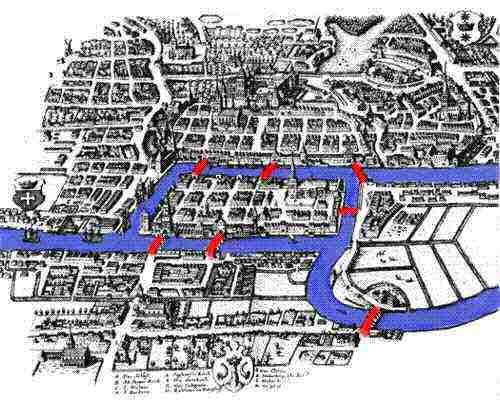
\includegraphics[width=0.3\textwidth]{chapters/konigsberg.jpg}
    \caption{The Seven Bridges of K\"onigsberg}
    \label{fig:konigsberg}
\end{figure}

Euler asked the question if one could cross each of the seven bridges exactly once and come back to the same side of the riverbank; this is formally considered as the first ever problem in graph theory.

Here, an \eax{Eulerian circuit} is defined, which is a closed path using every edge in the graph exactly once. A graph with an Eulerian circuit is termed an \eax{Eulerian graph}.

\begin{figure}[h]
    \centering
    \begin{tikzpicture}[scale=1.2,
        every node/.style={circle, draw=\subjectcolor!80!black, fill=\subjectcolor!40!white, inner sep=2pt}]
        
        % Nodes
        \node (A) at (0, 1.5) {A}; % North bank
        \node (B) at (0, 0) {B};   % South bank
        \node (C) at (2, 0.75) {C}; % Island (Kneiphof)
        \node (D) at (4, 0.75) {D}; % East bank or another land mass

        % Edges (bridges)
        \draw (A) -- (B);         % Bridge 1
        \draw (A) -- (C);         % Bridge 2
        \draw (A) -- (C);         % Bridge 3 (double line)
        \draw (B) -- (C);         % Bridge 4
        \draw (B) -- (C);         % Bridge 5 (double line)
        \draw (A) -- (D);         % Bridge 6
        \draw (C) -- (D);         % Bridge 7

    \end{tikzpicture}
    \caption{Graph Representation of the Seven Bridges of K\"onigsberg}
    \label{fig:konigsberg_graph}
\end{figure}
(Above graph to be fixed.)

\begin{theorem}
    A finite multigraph $G$ is Eulerian if and only if $G$ is connected and is a edge-disjoint union of cycle $G = C_{1} \cup C_{2} \cup \cdots \cup C_{m}$ where $C_{i}$'s are cycles with no common edges.
\end{theorem}

\begin{proof}
    Suppose $G = C_{1} \cup C_{2} \cup \cdots \cup C_{m}$ where $C_{i}$'s are edge-disjoint cycles. For $m = 2$, choose $v \in V(C_{1}) \cap V(C_{2})$; such a $v$ must exist or else the graph is disconnected. Starting at $v$, exhaust all edges in $C_{1}$ using the trivial Eulerian circuit and return to $v$. Do the same with $C_{2}$, and you have found the Eulerian circuit. Now apply the induction hypothesis; for an arbitrary $m$, choose $v \in V(C_{1} \cup C_{2} \cup \cdots \cup C_{m-1}) \cap V(C_{m})$. Again, such a $v$ must exist since $G$ is connected. Starting at $v$, exhaust all edges in $C_{1}$ using the trivial Eulerian circuit and return to $v$, then use the Eulerian circuit in $C_{1} \cup C_{2} \cup \cdots \cup C_{m-1}$ formed via the induction hypothesis.

    For the converse, an Eulerian circuit on the graph involves all edges and returns to the same vertex, so $G$ must be connected. To show the disjoint union of cycles, find a cycle in the Eulerian circuit; there must exist at least one since, if not, the circuit itself is a cycle. Delete the edges from this cycle, and join the starting vertex and ending vertex in of this cycle in the circuit. Repeat the same until the resulting Eulerian circuit is a cycle. The disjoint union of this cycle and the cycles removed is the starting circuit.
\end{proof}

One can show a better result.

\begin{theorem}
    A finite multigraph $G$ is Eulerian if and only if $G$ is connected and every vertex has an even degree.
\end{theorem}

\begin{proof}
    If $G$ is Eulerian, then $G$ is connected by the previous theorem, and $G = C_{1} \cup C_{2} \cup \cdots \cup C_{m}$, a union of disjoint cycles. Also, for $v \in V(G)$,
    \begin{align}
        \deg_{G}(v) = \sum_{i=1}^{m} \deg_{C_{i}}(v) = 2 \left( \sum_{i=1}^{m} \1_{\{v \in C_{i}\}} \right).
    \end{align}
    Thus, $\deg_{G}(v)$ is even for all $v \in V(G)$.

    For the converse implication, assume $G$ is connected and every vertex has an even degree. We will show that $G$ is Eulerian. Start by choosing any cycle $C_{1}$ in $G$. Remove the edges of $C_{1}$ from $G$ to form a subgraph $G'$. Since every vertex in $G$ has even degree, removing the edges of $C_{1}$ leaves every vertex in $G'$ with even degree. If $G'$ is connected, repeat the process to find another cycle $C_{2}$ in $G'$. Continue this process until no edges remain. If $G'$ is disconnected at any step, then each connected component of $G'$ must also have all vertices of even degree. By the same argument, we can find cycles in each connected component and remove their edges. Eventually, all edges of $G$ are partitioned into disjoint cycles. Since $G$ is connected, these cycles can be combined into a single Eulerian circuit by appropriately traversing edges between cycles. Thus, $G$ is Eulerian.
\end{proof}

\section{Adjacency}

For a simple graph $G = (V,E)$, an \eax{adjacency matrix} can be defined of dimension $\# V \times \# V$, with $a_{v,w} = 1$ if $vw \in E$, and $a_{v,w} = 0$ otherwise. For a multigraph, $a_{v,w}$ is the number of edges between vertices $v$ and $w$. Similarly, for a directed graph, $a_{v,w} = 1$ if $vw \in E$ and $a_{w,v} = 0$ otherwise. For an undirected graph, the adjacency matrix $A$ is symmetric and consists of only 1's and 0's. 

\begin{figure}[h]
    \centering
    \begin{tikzpicture}[scale=1.2,
        every node/.style={circle, draw=\subjectcolor!80!black, fill=\subjectcolor!40!white, inner sep=2pt}]
        
        % Nodes with slight deviations
        \node (A) at (0.1, 1.6) {$v_{1}$};
        \node (B) at (1.6, 1.4) {$v_{2}$};
        \node (C) at (-0.1, -0.1) {$v_{3}$};
        \node (D) at (1.4, 0.1) {$v_{4}$};

        % Edges
        \draw (A) -- (B);
        \draw (A) -- (C);
        \draw (B) -- (D);
        \draw (C) -- (D);
        \draw (B) -- (C);

    \end{tikzpicture}
    \caption{A simple graph with four vertices}
    \label{fig:graph_example}
\end{figure}
The adjacency matrix for the graph in Figure~\ref{fig:graph_example} is given as
$
A =
\begin{bmatrix}
0 & 1 & 1 & 0 \\
1 & 0 & 1 & 1 \\
1 & 1 & 0 & 1 \\
0 & 1 & 1 & 0
\end{bmatrix}
$. For two graphs $G_{1}$ and $G_{2}$ to be isomorphic, one can show that $A(G_{1})$ must be similar to $A(G_{2})$. Moreover, to count the number of walks from $v$ to $w$ of length $k$, one can use the $k$-th power of the adjacency matrix: the entry $(i,j)$ of $A^{k}$ gives the number of walks of length $k$ from vertex $v_{i}$ to vertex $v_{j}$.

\textit{August 28th.}
\begin{theorem}
    Let $G = (V,E)$ be a simple graph with $n$ vertices $V = \{1,2,\ldots,n\}$ and adjacency matrix $A$. Then the $(i,j)^{\text{th}}$ entry of $A^{k}$ gives the number of walks of length $k$ from vertex $i$ to vertex $j$.
\end{theorem}

\begin{proof}
    $k = 1$ is trivial, as a walk of length $1$ is just showing there exists an edge between the two vertices. Let $k = 2$. Then the $(i,j)^{\text{th}}$ entry of $A^{2}$ is given as
    \begin{align}
        (A^{2})_{i,j} = \sum_{m=1}^{n} a_{im} a_{mj}
    \end{align}
    where $a_{ij}$ is 1 if $i$ and $j$ are neighbours and zero otherwise. Thus, $a_{im}a_{mj}$ represents if vertex $m$ is an immediate intermediate vertex between $i$ and $j$. Thus, the number of walks of length 2 from $i$ to $j$ is equal to the number of such intermediate vertices $m$.

    Assume the result holds for an arbitrary $k$; that is, $(A^{k})_{i,j}$ gives the number of walks from $i$ and $j$ of length $k$. Then, for $k+1$, we have
    \begin{align}
        (A^{k+1})_{i,j} = \sum_{m=1}^{n} (A^{k})_{i,m} a_{mj}.
    \end{align}
    Any walk from $i$ to $j$ must have a neighbour of $j$ at the $k^{\text{th}}$ step. By the induction hypothesis, $(A^{k})_{i,m}$ represents the number of walks from $i$ to $m$ of length $k$. Thus, the total number of walks from $i$ to $j$ of length $k+1$ is the sum over all possible intermediate vertices $m$.
\end{proof}

\begin{theorem}
    Let $\lambda_{1},\ldots,\lambda_{n}$ be the eigenvalues of $A(G)$ where $G = (V,E)$ is a simple graph. Then the number of closed walks of length $k$ is given by $\sum_{i=1}^{n} \lambda_{i}^{k}$.
\end{theorem}
\begin{proof}
    The number of such closed walks of length $k$ is, clearly, $\tr A^{k}$. The eigenvalues of $A^{k}$ are $\lambda_{1}^{k},\ldots,\lambda_{n}^{k}$, and the trace is the sum of all eigenvalues; the result immediately follows.
\end{proof}

\begin{remark}
    \begin{itemize}
        \item For $k = 2$, $\frac{1}{2}\tr A^{2}$ provides the number of edges in the graph.
        \item For $k = 3$, $\frac{1}{6}\tr A^{3}$ provides the number of triangles in the graph.
    \end{itemize}
\end{remark}

\begin{example}
    $G$ is connected if and only if the largest eigenvalue of $A$ has multiplicity 1. This is known as the \eax{Perron-Frobenius theorem} will be taken as granted for now, without providing a proof.
\end{example}

\begin{proposition}
    For any eigenvalue $\lambda$ of $G = (V,E)$, it holds that $\abs{\lambda} \leq \max_{v \in G} \deg(v)$.
\end{proposition}
\begin{proof}
    Pick a corresponding eigenvector $x \neq 0$ with $Ax = \lambda x$, where $A$ is the adjacency matrix. Pick $x_{j} = \norm{x}_{\infty} = \max_{i} \abs{x_{i}}$. Then we have
    \begin{align}
        \abs{\lambda}\abs{x_{j}} = \abs{\lambda x_{j}} = \abs{\sum_{i=1}^{n} A_{ji} x_{i}} \leq \sum_{i=1}^{n} A_{ji} \abs{x_{i}} \leq \abs{x_{j}} \sum_{i=1}^{n} A_{ji} = \abs{x_{j}} \deg (j) \implies \abs{\lambda} \leq \deg (j) \leq \max_{v \in G} \deg(v).
    \end{align}
\end{proof}

\begin{proposition}
    Let spectrum of $G = \{\lambda_{1},\ldots,\lambda_{n}\}$ be the list of eigenvalues where $\lambda_{1} \leq \lambda_{2} \leq \cdots \leq \lambda_{n}$. Then
    \begin{align}
        \frac{1}{n}\sum_{v \in G} \deg(v) \leq \lambda_{n} \leq \max_{v \in G} \deg(v).
    \end{align}
\end{proposition}

\begin{proof}
    Let $e = (1\;1\;\cdots\;1)^{t}$, and let $d = Ae = (\deg(v_{1})\;\deg(v_{2})\;\cdots\;\deg(v_{n}))^{t}$. Then $e^{t}Ae = ed = \sum_{v \in G} \deg(v)$. Then $\sup_{\norm{x}=1}\ip{x,Ax} = \lambda_{\max}(A) \geq \frac{e^{t}}{\sqrt{n}} A \frac{e}{\sqrt{n}} = \frac{1}{n}\sum_{v \in G} \deg(v)$. The second inequality is just the one above.
\end{proof}

\begin{theorem}
    A finite multigraph $G$ is Eulerian if and only if $G$ is connected and every vertex has an even degree.
\end{theorem}
\begin{proof}
    If $G$ is Eulerian, then it is connected and every vertex has an even degree by definition. Conversely, suppose $G$ is connected and every vertex has an even degree. Take `a' longest trail, one where edges are not repeated, starting at $x \in V(G)$. We claim that this trail is actually closed. Let, if possible, the endpoint be $y \neq x$. There must have been an ``entering'' edge followed by an ``exiting'' edge. In the last step, one has entered $y$ but never exited it. So, an odd number of edges incident with $y$ appear in this trail. As $\deg(y)$ is even, there must be an unused edge incident with $y$. If we append that edge to the trail, we have a longer trail, contradicting our assumption.

    We make another claim that this trail exhausts all edges. To show this, start by deleting all edges appearing in this trail. Assume that the graph so-obtained has at least one edge. In the trail, $T$, if a vertex $y$ appears all its incident edges must also appear. Let $z$ be a vertex not appearing on $T$. Then none of the vertices in $T$ are neighbours of $z$, showing $G$ not connected which is a contradiction.
\end{proof}


\subsubsection{Hamiltonian Graphs}
\textit{August 29th.}

\begin{definition}
    A cycle in $G = (V,E)$ is said to be a \eax{Hamiltonian cycle} if the vertices in the cycle are all distinct, except the starting and ending vertices, and all vertices are exhausted. A simple graph with a Hamiltonian cycle is termed a \eax{Hamiltonian graph}.
\end{definition}

\begin{example}
    \begin{itemize}
        \item Trivially, all polygons with $n$ vertices $C_{n}$ are Hamiltonian graphs.
        \item The complete graph $K_{n}$ is Hamiltonian for all $n \geq 3$.
    \end{itemize}
\end{example}

If $G = (V,E)$ is a graph, then a \eax{subgraph} $H = (V(H),E(H))$ is such that $V(H) \subseteq V(G)$ and $E(H) \subseteq V(H)$ where $E(H)$ are edges connecting vertices in $V(H)$. A \eax{spanning subgraph} is such that $V(H) = V(G)$. We note that $G$ is Hamiltonian if and only if $C_{n}$ is a spanning subgraph of $G$.

Our goal now is to find a characterizing condition for Hamiltonian graphs (similar to the characterization of Eulerian graphs), and if a graph is Hamiltonian, then finding the (a) Hamiltonian cycle. The proof of providing a characterization is out of the scope of this course, while the latter problem is NP-hard and not always computationally tactible.


\begin{definition}
    The \eax{Hamiltonian closure of a graph} $G$, denoted by $\cl(G)$, is the graph obtained by repeatedly adding an edge between non-adjacent vertices $u,v$ such that $\deg(u)+\deg(v) \geq n = \#V(G)$.
\end{definition}

\begin{proposition}
    With $\#V(G) = n \geq 3$, let $G$ be a simple graph. If $\deg(v) \geq \frac{n}{2}$ for all $v \in V(G)$, then $G$ is Hamiltonian.
\end{proposition}

\begin{lemma}
    A graph $G$ is Hamiltonian if and only if $\cl(G)$ is Hamiltonian.
\end{lemma}
\begin{proof}
    If $G$ is Hamiltonian, then clearly $\cl(G)$ is Hamiltonian since adding edges cannot remove Hamiltonian cycles. Conversely, suppose $\cl(G)$ is Hamiltonian. Assume the contrary that there exists $G$ with $\#V(G) = n$ and $u$ an $v$ are \textit{not} neighbours in $G$ with $\deg(u)+\deg(v) \geq n$, but $G$ is not Hamiltonian. $G+uv$ is Hamiltonian, however. Suppose the intermiedate graphs obtained to get the closure are given as
    \begin{align}
        G = G_{0} \subseteq G_{1} \subseteq G_{2} \subseteq \cdots \subseteq G_{t} = \cl(G)
    \end{align}
    where $\cl(G)$ is Hamiltonian. Then every Hamiltonian cycle in $G+uv$ must contain the edge $uv$. Let this Hamiltonian cycle be $(v,v_{1},\ldots,v_{n-1},v_{n} = u,v_{n+1}=v)$. Let $P = \{v_{i} \mid 2 \leq i \leq 2 \text{ and } v_{1}v_{i} \in E(G)\}$ and $Q = \{v_{i} \mid 2 \leq i \leq n \text{ and } v_{i-1}v_{n} \in E(G)\}$ ($P$ and $Q$ are defined with respect to $G$ and \textit{not} $G+uv$). Then $\#P = \deg(v)$, $\#Q = \deg(v_{n})$, and $\#P+\#Q = \deg(u) + \deg(v) \geq n$. Moreover, $P \cup Q \subseteq \{v_{2},\ldots,v_{n}\}$. $P \cap Q$ is non-empty since
    \begin{align}
        \#(P \cup Q) = \#P + \#Q - \#(P \cap Q) \geq n-\#(P \cap Q) \implies \#(P \cap Q) \geq n-\#(P \cup Q) \geq 1.
    \end{align}
    Thus, there exists some $v_{i} \in P \cap Q$ with $2 \leq i \leq n$, that is, $v_{1}v_{i} \in E(G)$ and $v_{i-1}v_{n} \in E(G)$. Then the cycle $(v=v_{1},v_{i},v_{i+1},\ldots,v_{n}=u,v_{i-1},v_{i-2},\ldots,v_{2},v_{1})$ is a Hamiltonian cycle not using the added edge $uv$---a contradiction.
\end{proof}

\section{Bipartite Graphs}

A simple graph $G = (V,E)$ is said to be bipartite if there exists a partition of $V(G)$ as $V = V_{1} \sqcup V_{2}$ such that no pairs of vertices in $V_{1}$ are edges, and no pairs of vertices in $V_{2}$ are edges; that is, there exist $V_{1},V_{2} \subseteq V$ such that
\begin{align}
    V_{1} \cap V_{2} = \emptyset,\; V_{1} \sqcup V_{2} = V,\; E \subseteq V_{1} \times V_{2}.
\end{align}

\textit{September 2nd.}

\begin{theorem}[\eax{Kőnig's theorem}]
    A graph $G$ is bipartite if and only if it has no odd cycles.
\end{theorem}
\begin{proof}
    Suppose $G$ is bipartite with the required vertex sets $V_{1} \sqcup V_{2} = V(G)$. Take a cycle of length $n$ in $G$ and suppose it is an odd cycle, say $C = (v_{1},v_{2},\ldots,v_{2k},v_{2k+1},v_{1})$ where $k \geq 1$. Without the loss of generality, assume $v_{1} \in V_{1}$. Since a vertex's neighbours must be in a different vertex set, we have $v_{2} \in V_{2}$. Proceeding inductively, we have $\{v_{1},v_{3},\ldots,v_{2k+1}\} \subseteq V_{1}$ and $\{v_{2},v_{4},\ldots,v_{2k}\} \subseteq V_{2}$. But $v_{1}v_{2k+1} \in E(G)$, which is a contradiction since both $v_{1}$ and $v_{2k+1}$ are in $V_{1}$. Thus, every cycle in $G$ must be even.

    For the converse, let $v_{0} \in V$ and put it in a vertex set $V_{1}$. Put the neighbours of $v_{0}$ in $V_{2}$, that is, $N(v_{0}) \subseteq V_{2}$. We note that for $w_{1},w_{2} \in N(v_{0})$, there cannot be the edge $w_{1}w_{2}$, since having so would make $(v_{0},w_{1},w_{2},v_{0})$ an odd cycle. Now put the neighbours of $N(v_{0})$ in $V_{1}$, that is, $N(N(v_{0})) \subseteq V_{1}$. Note that $v_{0} \in N(N(v_{0}))$. Again, for $w_{1},w_{2} \in N(N(v_{0}))$, there cannot be the edge $w_{1}w_{2}$ since having so would make $(v_{0},\ast_{1},w_{1},w_{2},\ast_{2},v_{0})$ an odd cycle, where $\ast_{1},\ast_{2}$ are neighbours of $w_{1}$ and $w_{2}$ respectively, and both are in $N(v_{0}) \subseteq V_{1}$. Proceeding so, we have $V_{1} = \{v \in V \mid d_{G}(v_{0},v) \text{ is even }\}$ and $V_{2} = \{v \in V \mid d_{G}(v_{0},v) \text{ is odd }\}$. This shows bipartition for a connected $G$. Note that $G$ is bipartite if and only if every connected component of $G$ is bipartite (a \eax{connected component} of $G$ is an equivalence relation on $V$, with $x \sim y$ if and only if there exists a path from $x$ to $y$ or $x = y$). If we find a bipartition of every connected component with $V_{1}^{(i)},V_{2}^{(i)}$ where $i$ signifies the $i^{\text{th}}$ connected component, then defining
    \begin{align}
        V_{1} = \bigsqcup_{i=1}^{k} V_{1}^{(i)},\quad V_{2} = \bigsqcup_{i=1}^{k} V_{2}^{(i)}
    \end{align}
    results in the required bipartition. Coming back to the definition of $V_{1}$, all vertices even length away from $v_{0}$, and $V_{2}$, all vertices odd length away from $v_{0}$, we claim that no two vertices in $V_{1}$ are neighbours. Let us assume for contradiction that there exist $v,w \in V_{1}$ which are neighbours. Let $P$ be the shortest path from $v_{0}$ to $v$ and $P'$ be the shortest path from $v_{0}$ to $w$. Then $(v_{0},P',w,v,P,v_{0})$ is a walk of odd length which is a contradiction. Hence, any $v$ and $w$ in $V_{1}$ cannot be neighbours. Similarly, one can show fro $V_{2}$.
\end{proof}

$K_{m,n}$ denotes the \eax{complete bipartite graph} with $m$ vertices in one vertex set and $n$ vertices in the other vertex set. Here, $uv$ is an edge in $K_{m,n}$ if and only if $u$ and $v$ are in different vertex sets. Thus the number of edges in $E(K_{m,n})$ is $mn$.

\begin{corollary}
    A bipartite graph has no triangles.
\end{corollary}

To guarantee a triangle, how many edges must have a simple graph $G$ have? We have the following theorem.

\begin{theorem}[\eax{Mantel's theorem}]
    If $G$, with $\#V(G) = n$, has more than $\floor{\dfrac{n^{2}}{4}}$ edges, then $G$ contains a triangle.
\end{theorem}

\begin{proof}[Alternate proof]
    Consider $G$ with no triangles, with $m$ edges and $n$ vertices. Let $x$ and $y$ be two vertices in $G$ such that $xy \in E(G)$. Then $\deg(x) + \deg(y) \leq n$ since each vertex in $G$ can only be connected to one of $x$ or $y$; otherwise, if a vertex $z$ were adjacent to both, the set $\{x, y, z\}$ would form a triangle. Now observe that
    \begin{align}
        \sum_{xy \in E(G)} \left( \deg(x) + \deg(y) \right) &\leq m \cdot n.
    \end{align}
    On the other hand, each degree appears in this sum once for each incident edge, so:
    \begin{align}
        \sum_{xy \in E(G)} \left( \deg(x) + \deg(y) \right) &= \sum_{v \in V(G)} \deg(v)^2 \leq mn.
    \end{align}
    Applying the Cauchy-Schwarz inequality results in
    \begin{align}
        \sum_{v \in V(G)} \deg(v)^2 \geq \frac{1}{n} \left( \sum_{v \in V(G)} \deg(v) \right)^2 = \frac{(2m)^2}{n}.
    \end{align}
    Combining the two inequalities gives
    \begin{align}
        \frac{4m^2}{n} \leq m n \implies m \leq \frac{n^2}{4}.
    \end{align}
    Hence, the number of edges is at most $\left\lfloor \frac{n^2}{4} \right\rfloor$, as desired.
\end{proof}

\subsection{Coloring}
\textit{September 4th.}

A \eax{proper coloring} of a graph $G$ is a mapping $f:V \to C$, where $C$ is a finite set of a colors, such that for every edge $uv \in E(G)$, we have $f(u) \neq f(v)$. In other words, adjacent vertices must be assigned different colors. The \eax{chromatic number} $\chi(G)$ of a graph $G$ is the smallest number of colors needed for a proper coloring of $G$, that is, the minimal cardinality of $C$ required. For a planar graph $G$, $\chi(G)$ is at most 4.

One also has the \eax{chromatic polynomial} $P_{G}(k)$, or $P(G,k)$, which specifies the number of proper $k$-colorings of $G$ for a given $k$. From here, one can define
\begin{align}
    \chi(G) \defeq \min\{k \mid P(G,k) > 0\}.
\end{align}

\begin{proposition}[The \eax{deletion-contraction principle}]
    For any edge $e \in E(G)$, $G$ a graph,
    \begin{align}
        P(G,k) = P(G-e,k)-P(G\setminus e,k)
    \end{align}
    holds, where $G-e$ is the graph obtained by removing the edge $e$ from $G$ (termed deletion), and $G\setminus e$ is the graph obtained by joinin the vertices of edge $e$ (termed contraction).
\end{proposition}
\begin{proof}
    The proof is left as an exericse to the reader.
\end{proof}
The following are some properties of $P(G,x)$.
\begin{enumerate}
    \item $P(G,x)$ is a monic polynomial of degree $\#V(G)$.
    \item $\chi(G) = \min\{k \in \N \mid P(G,k) > 0\}$.
    \item The constant term of the polynomial, $a_{0}$, is zero.
    \item One has either $\sum_{i=1}^{n} a_{i} = 0$ or $P(G,x) = x^{n}$.
    \item $a_{n-i} = (-1)^{i}\abs{a_{n-i}}$.
    \item $a_{n-1} = -\#E(G)$.
\end{enumerate}

\begin{proof}
    We induct on $\#E$. Look at the base, $D_{n}$, a graph with $n$ vertices and no edges. Then $P(D_{n},x) = x^{n}$, a monic polynomial of degree $1$. For any graph $G$, we have $P(G,k)=P(G-e,k)-P(G\setminus e,k)$. By the induction hypothesis, $P(G-e,k)$ is a monic polynomial of degree $n$, and $P(G\setminus e, k)$ is monic polynomial of degree $n-1$. Thus, $P(G,k)$ is one too. The second property is by definition. The third statement follows the same argument as the first statement.

    For the fourth statement, note that $P(G,1) = 0$ if there is at least one edge. By induction, one can see that $\sum_{i=1}^{n} a_{i} = 0$, unless no edge is present, in which case $P(G,x) = P(D_{n},x) = x^{n}$. Fifth and sixth statements also follow an argument by induction
\end{proof}

\begin{theorem}
    The chromatic polynomial of a graph $G = (V,E)$ can be written in the form
    \begin{align}
        P(G,k) = \sum_{X \subseteq E} (-1)^{\#X}x^{\beta_{0}(X)}
    \end{align}
    where $\beta_{0}(X)$ denotes the number of connected components of the subgraph $(V,X)$.
\end{theorem}
Thus, to find the coefficient of $x^{m}$, one must collect all subgraphs with $m$ connected components. Let $k_{E}$ denote the number of spanning subgraphs of $G$ with $m$ connected components and even number of edges, and let $k_{O}$ denote the number of spanning subgroups of $G$ with $m$ connected components and odd number of edges. Then the coefficient of $x^{m}$ comes out to be $k_{E}-k_{O}$. In the case where $m = n$, we have $k_{E} = 1$ and $k_{O} = 0$.

\begin{proof}
    Here, $P(G,k) = k^{n} - \#(IC)$, where $IC$ is the number of improper colorings. Denote, for an edge $e = uv$, $B_{e} = \{c \in IC \mid c(u) = c(v)\}$. Then
    \begin{align}
        P(G,k) = k^{n} - \abs{\bigcup_{e \in E} B_{e}} = k^{n} - \sum_{X \neq \emptyset,\;X \subseteq E} (-1)^{\#X}\abs{\bigcap_{e \in X} B_{e}}
    \end{align}
    via the principle of inclusion-exclusion. Let $X = \{e_{1},\ldots,e_{k}\} \subseteq E$ with $e_{i} = u_{i}v_{i}$. Then
    \begin{align}
        \bigcap_{e \in X} B_{e} = \{c:V \to \{1,2,\ldots,k\} \mid c(u_{i}) = c(v_{i}) \text{ for all } i\} = k^{\beta_{0}(x)}
    \end{align}
    since the function $c$ has to be constant on each connected component of $(V,X)$. Hence,
    \begin{align}
        P(G,k) = k^{n} - \sum_{X \neq \emptyset,\;X \subseteq E} (-1)^{\#X} k^{\beta_{0}(X)}.
    \end{align}
\end{proof}

\section{Trees and Cayley's}

\textit{September 16th.}

\begin{definition}
    A graph $G$ with no simple cycles is called a \eax{forest}. A connected forest is called a \eax{tree}; essentially, a tree is a connected graph with no simple cycles.
\end{definition}

\begin{lemma}
    A finite tree on $n$ vertices, for $n \geq 2$, has at least two vertices of degree 1.
\end{lemma}
The vertex in a tree with degree 1 is called a \eax{leaf}.
\begin{proof}
    Pick the longest path in the tree $T$, say $v_{0}v_{1}\cdots v_{k}$. We claim that both $v_{0}$ and $v_{k}$ are leaves. If not, say $\deg v_{0} \geq 2$, then there exists $u \neq v_{1}$ such that $uv_{0} \in E(T)$. If $u$ is not in the path, then $uv_{0}v_{1}\cdots v_{k}$ is a longer path, contradicting our assumption. If $u$ is in the path, then there exists $uv_{0}v_{1}\cdots v_{i}u$ which is a simple cycle, contradicting the definition of a tree. Thus, $v_{0}$ must have degree 1. Similarly, one can show for $v_{k}$.
\end{proof}

\begin{lemma}
    A graph $G$ with $n$ vertices is a tree if and only if it is connected and has $n-1$ edges.
\end{lemma}
\begin{proof}
    If $G$ is a tree, then it is connected by definition. We induct on $n$. The base case $n = 1$ is trivial. Assume the result holds for all trees with up to $n-1$ vertices. Let $G$ be a tree with $n$ vertices. By the previous lemma, there exists a leaf $v$ in $G$. Remove $v$ and the edge incident with it to form a subgraph $G'$. Then $G'$ is a tree with $n-1$ vertices, and by the induction hypothesis, it has $(n-1)-1 = n-2$ edges. Thus, $G$ has $(n-2)+1 = n-1$ edges.

    For the converse, start with an $n$-vertex graph $G$. If $G$ contains a simple cycle, then removing an edge from that cycle leaves the graph connected; repeat until there are no such cycles. After (finitely) many steps, we end up with a tree, which we have shown to have $n-1$ edges. This meas that the original graph $G$, which had at least one cycle, must have had more than $n-1$ edges. 
\end{proof}

Similarly, one can show that $G$ is a forest if and only if it has $n-\beta_{0}(G)$ edges, where $\beta_{0}(G)$ is the number of connected components of $G$.

\begin{definition}
    A \eax{labelled tree} on $[n] = \{1,2,\ldots,n\}$ is a tree with vertex set $[n]$. Two labelled trees are considered distinct if they are not isomorphic via an isomorphism that preserves the labels.
\end{definition}

\textit{September 18th.}

\begin{theorem}[\eax{Cayley's theorem}]
    The number of labelled trees on $[n]$ is $n^{n-2}$.
\end{theorem}
\begin{proof}
    We will show a bijection between the set of labelled trees on $[n]$ and $[n]^{n-2}$, the set of all sequences of length $n-2$ with entries from $[n]$. For a labelled tree $T$ on vertex set $[n]$, generate a sequence of labelled trees $T_1, T_2, \ldots, T_{n-1}$ inductively as follows: let $T_1 = T$, and obtain $T_2$ by removing the leaf with the smallest label from $T_1$ along with its incident edge. Continue this process: at each step, remove the leaf with the smallest label from the current tree and its incident edge. This process terminates with $T_{n-1}$, which is a tree on two vertices. Thus, each $T_i$ is a labelled tree on $n - i + 1$ vertices.

    Let $x_i$ denote the leaf removed from $T_i$ (i.e., the leaf of $T_i$ with the smallest label), and let $y_i$ denote its unique neighbor in $T_i$. Define a sequence $(y_1, y_2, \ldots, y_{n-2})$, which we call the \eax{Prüfer code} of the tree $T$. Since at each step the removed leaf and its neighbor are well-defined, and since the process continues for $n - 2$ steps, this produces a sequence of length $n - 2$ with entries from $[n]$. Hence, every labelled tree on $[n]$ gives rise to a unique Prüfer code in $[n]^{n-2}$.

    To show that this map is a bijection, it remains to show that every sequence in $[n]^{n-2}$ corresponds to a unique labelled tree on $[n]$. Given a sequence $(y_1, y_2, \ldots, y_{n-2})$ in $[n]^{n-2}$, we reconstruct the tree as follows:
    \begin{enumerate}
        \item Initialize the degree of each vertex $v \in [n]$ by $\deg(v) = 1 + \#\{i \mid y_i = v\}$, which counts the number of times $v$ appears in the sequence plus one (show this to be true).
        \item For $i = 1$ to $n - 2$, find the smallest vertex $x_i$ such that $\deg(x_i) = 1$. Add the edge $(x_i, y_i)$ to the tree, and decrease both $\deg(x_i)$ and $\deg(y_i)$ by 1.
        \item After processing all entries in the sequence, two vertices remain with degree 1. Connect these two vertices to complete the tree.
    \end{enumerate}

    This algorithm constructs a unique labelled tree from any given Prüfer code. Since both the encoding and decoding procedures are well-defined and inverse to one another, the correspondence is a bijection between the set of labelled trees on $[n]$ and $[n]^{n-2}$.
\end{proof}
A few key observations may be inferred:
\begin{enumerate}
    \item If $(y_{1},y_{2},\ldots,y_{n-2})$ is the Prüfer code of tree $T$, then $(y_{2},\ldots,y_{n-2})$ is the Prüfer code of the tree $T_{2}$.
    \item The degree of a vertex $i$ is $d_{i} = \sum_{j=1}^{n-2} \1_{[y_{j}=i]} + 1$.
    \item The leaf $x_{k} = \min_{i \in [n]}\{i \mid i \notin \{x_{1},\ldots,x_{k-1},y_{k},y_{k+1},\ldots,y_{n-2}\}\}$.
\end{enumerate}
Note that 1.~follows from the definition, and 2.~can be shown as a result of induction.

\begin{theorem}[The \eax{tree counting theorem}]
    The number of labelled spanning trees on $n$ vertices with degree sequence $(d_{1},d_{2},\ldots,d_{n})$ is given by
    \begin{align}
        \binom{n-2}{d_{1}-1,\ldots,d_{n}-1} = \frac{(n-2)!}{(d_{1}-1)!(d_{2}-1)!\cdots(d_{n}-1)!}.
    \end{align}
\end{theorem}
\begin{proof}
    In the Prüfer code of a labelled tree $T$, a vertex $i$ appears exactly $d_{i}-1$ times. Thus the counting problem is equivalent to the number of Prüfer codes which contain $d_{i}-1$ copies of $i$. This is given by the multinomial coefficient above.
\end{proof}

\section{Ramsey Theory}

In any graph $G$ on $6$ vertices, either $K \subseteq G$ or $K_{3} \subseteq \overline{G}$, where $\overline{G}$ is the complement of $G$. $G$ and $\overline{G}$ cannot both be triangle-free. Equivalently, any edge-colouring of $K_{6}$ with two colours must have a monochromatic triangle.

\begin{definition}
    The \eax{Ramsey number} $R(m,n)$ is defined as
    \begin{align}
        R(m,n) = \inf \{t \mid \text{ for any } G \subseteq K_{t}, \text{ either } K_{m} \subseteq G \text{ or } K_{n} \subseteq \overline{G}\}
    \end{align}
\end{definition}

One can easily see that $R(m,2) = m$ and $R(m,n) = R(n,m)$, and $R(m,n) < \infty$ for all $m,n \in \N$.

\begin{lemma}
    $R(m,n) \leq R(m-1,n) + R(m,n-1)$ for all $m,n \geq 2$.
\end{lemma}
\begin{proof}
    Let $t = R(m-1,n) + R(m,n-1)$ and consider $v \in V(K_{t})$, joined to $t-1$ other vertices. Bicolour all edges red or blue. Let $P$ be the set of all vertices connected to $v$ by a red edge, and let $Q$ be the set of all vertices connected to $v$ by a blue edge. Then $\#P + \#Q = p+q = t-1$. Thus either $p \geq R(m-1,n)$ or $q \geq R(m,n-1)$. If $p \geq R(m-1,n)$, then either there is a red $(m-1)$-clique with vertices in $P$ or there is a blue $n$-clique with vertices in $P$. In the former case, adding $v$ gives a red $m$-clique; in the latter case, we are done. Similarly, if $q \geq R(m,n-1)$, then either there is a red $m$-clique with vertices in $Q$ or there is a blue $(n-1)$-clique with vertices in $Q$. In the latter case, adding $v$ gives a blue $n$-clique; in the former case, we are done.
\end{proof}

\begin{lemma}
    $R(n,n) \leq 4^{n}$ for all natural $n$.
\end{lemma}
\begin{proof}
    Using the above inequality, a proof by induction on $n$ suffices.
\end{proof}

\begin{lemma}
    $R(n,n) > \floor{2^{n/2}}$ for all natural $n$.
\end{lemma}
\begin{proof}
    Let $t = \floor{2^{n/2}}$. There is an edge colouring of $K_{t}$ such that there is no monochromatic $K_{n}$; we wish to show this. Set of all possible colourings on $K_{t}$ is $\Omega_{t} = E(K_{t})^{\{R,B\}}$. Let $f:E(K_{t}) \to \{R,B\}$ be such a colouring. THe number of such functions is clearly $2^{\binom{t}{2}}$. Let $A_{t} = \{f \in \Omega_{t} : f \text{ has no monochromatic } n-\text{clique}\}$. $A_{t} \neq\emptyset$ and $\Omega_{t} \setminus A_{t} \neq \Omega_{t}$. If $f \notin A_{t}$, there exists $S \subseteq [t]$ and $\#S = n$ such that $f$ is constant on $E_{S}$. Thus,
    \begin{align}
        \Omega_{t} \setminus A_{t} = \bigcup_{S \subseteq [t],\; \#S = n} \{f \in \Omega_{t} : f \text{ is constant on } E_{S}\}.
    \end{align}
    We now look at the probability of a random colouring $X$ being in $\Omega_{t} \setminus A_{t}$.
    \begin{align}
        P(X \in \Omega_{t} \setminus A_{t}) \leq \sum_{S \subseteq [t],\; \#S = n} P(X|_{E_{S}} = R) + P(X|_{E_{S}} = B) = \sum_{S \subseteq [t],\; \#S = n} \frac{2}{2^{\binom{n}{2}}} = \binom{t}{n} \frac{1}{2^{\binom{n}{2}-1}}.
    \end{align}
    
\end{proof}
\chapter{CONVERGENCE}

\section{Types of Convergence}

\textit{September 26th.}

Let $\{X_{n}\}_{n \geq 1}$ be a sequence of random variables defined on a probability space $(\Omega, \cF, P)$ and let $X$ be another random variable defined on the same probability space. 

\begin{definition}
    Notion of \eax{convergence in probability}: We say that $X_{n}$ converges to $X$, $X_{n} \xrightarrow{P} X$, if for every $\varepsilon > 0$,
    \begin{align}
        P(\abs{X_{n}-X} \geq \varepsilon) \to 0 \text{ as } n \to \infty.
    \end{align}
\end{definition}

An example is the \eax{weak law of large numbers} which states that if $X_{1}, X_{2}, \ldots$ are independent and identically distributed random variables with mean $\mu$, then the sample average $\overline{X}_{n} = \frac{1}{n} \sum_{i=1}^{n} X_{i}$ converges in probability to $\mu$.

\begin{definition}
    Notion of \eax{almost sure convergence}: We say that $X_{n}$ converges to $X$ almost surely, $X_{n} \xrightarrow{a.s.} X$, if 
    \begin{align}
        P\left(\{\omega \in \Omega \mid \lim_{n \to \infty} X_{n}(\omega) = X(\omega)\}\right) = 1.
    \end{align}
\end{definition}

An example is the \eax{strong law of large numbers} which states that if $X_{1}, X_{2}, \ldots$ are independent and identically distributed random variables with mean $\mu$, then the sample average $\overline{X}_{n} = \frac{1}{n} \sum_{i=1}^{n} X_{i}$ converges almost surely to $\mu$.

\begin{definition}
    Notion of \eax{convergence in distribution}: We say that $X_{n}$ converges to $X$ in distribution, $X_{n} \xrightarrow{d} X$, if
    \begin{align}
        F_{X_{n}}(x) \to F_{X}(x) \text{ at all points } x \text{ where } F_{X} \text{ is continuous},
    \end{align}
    where $F_{X_{n}}$ and $F_{X}$ are the cumulative distribution functions of $X_{n}$ and $X$ respectively.
\end{definition}

An example is the \eax{central limit theorem} which states that if $X_{1}, X_{2}, \ldots$ are independent and identically distributed random variables with mean $\mu$ and variance $\sigma^{2}$, then the standardized sum $\frac{\sum_{i=1}^{n} (X_{i} - \mu)}{\sigma \sqrt{n}}$ converges in distribution to a standard normal random variable as $n \to \infty$.

\begin{lemma}[\eax{Borel-Cantelli lemma}]
    Let $A_{1},A_{2},\ldots$ be a sequence of events in a probability space $(\Omega, \cF, P)$.
    \begin{enumerate}
        \item If the sum of the probability of the events $A_{n}$ is finite, i.e., $\sum_{n=1}^{\infty} P(A_{n}) < \infty$, then the probability that infinitely many of the events $A_{n}$ occur is zero, i.e., $P(\limsup_{n \to \infty} A_{n}) = 0$.
        \item If $\sum_{n=1}^{\infty} P(A_{n}) = \infty$ and the events $A_{n}$ are independent, then the probability that infinitely many of the events $A_{n}$ occur is one, i.e., $P(\limsup_{n \to \infty} A_{n}) = 1$.
    \end{enumerate}
\end{lemma}

\begin{theorem}[\eax{Slutsky's theorem}]
    Suppose $X_{n} \xrightarrow{d} X$ and $Y_{n} \xrightarrow{P} c$, where $c$ is a constant. Then
    \begin{enumerate}
        \item $X_{n} + Y_{n} \xrightarrow{d} X + c$,
        \item $X_{n}Y_{n} \xrightarrow{d} Xc$, and
        \item $\frac{X_{n}}{Y_{n}} \xrightarrow{d} \frac{X}{c}$, provided $c \neq 0$.
    \end{enumerate}
\end{theorem}

\begin{proof}
    With the conditions, one can show that the joint vector $(X_{n}, Y_{n})$ converges in distribution to $(X, c)$. The results then follow from the continuous mapping theorem, which states that for a continuous function $g$, $Z_{n} \xrightarrow{d} Z$ implies $g(Z_{n}) \xrightarrow{d} g(Z)$.
\end{proof}

\begin{corollary}
    If $X_{n} - Y_{n} \xrightarrow{P} 0$ and $X_{n} \xrightarrow{d} X$, then $Y_{n} \xrightarrow{d} X$.
\end{corollary}
\begin{proof}
    Work similarly as before, looking at the joint vector $(X_{n}-Y_{n},X_{n})$ and using the continuous mapping theorem with the function $g(x,y) = y - x$.
\end{proof}

Recall \eax{Markov's inequality} where for any random variable $X$ and $a > 0$, we have
\begin{align}
    P(X \geq a) \leq \frac{EX}{a}.
\end{align}
Replacing $X$ by $X^{2}$ and $a$ with $a^{2}$ gives
\begin{align}
    P(\abs{X} \geq a) \leq \frac{E[X^{2}]}{a^{2}}.
\end{align}
Finally, replacing $X$ by $\abs{X - E[X]}$ gives \eax{Chebyshev's inequality}:
\begin{align}
    P(\abs{X - EX} \geq a) \leq \frac{\Var(X)}{a^{2}}.
\end{align}

\begin{theorem}[\eax{Kinchin's weak law of large numbers}]
    Let $X_{1}, X_{2}, \ldots$ be a sequence of independent and indentically distributed random variables such that $EX_{i} = \mu$ exists and $\overline{X}_{n} = \frac{1}{n} \sum_{i=1}^{n} X_{i}$. Then $\overline{X}_{n} \xrightarrow{P} \mu$.
\end{theorem}

\begin{theorem}[\eax{Chebyshev's weak law of large numbers}]
    Let $X_{1}, X_{2}, \ldots$ be a sequence of random variables with $EX_{i} = \mu_{i}$ and $\Var(X_{i}) = \sigma_{i}^{2} < \infty$. Moreover, suppose $\Cov(X_{i},X_{j}) = 0$ for $i \neq j$. Then
    \begin{align}
        \frac{1}{n} \sum_{i=1}^{n} \sigma_{i}^{2} \to 0 \text{ as } n \to \infty \implies \overline{X}_{n} - \overline{\mu}_{n} \xrightarrow{P} 0,
    \end{align}
    where $\overline{\mu}_{n} = \frac{1}{n} \sum_{i=1}^{n} \mu_{i}$.
\end{theorem}

\begin{theorem}[\eax{Kolmogorov's strong law of large numbers}]
    Let $X_{1}, X_{2}, \ldots$ be a sequence of independent and identically distributed random variables such that $EX_{i} = \mu$ exists. Then $\overline{X}_{n} \xrightarrow{a.s.} \mu$.
\end{theorem}

\begin{theorem}[\eax{Lindeberg-levy central limit theorem}]
    Let $X_{1},X_{2},\ldots$ be a sequence of independent and identically distributed random variables with $EX_{i} = \mu$ and $\Var(X_{i}) = \sigma^{2} < \infty$. Then
    \begin{align}
        \frac{\overline{X}_{n} - \mu}{\sigma/\sqrt{n}} \xrightarrow{d} N(0,1).
    \end{align}
\end{theorem}

\subsection{Consistency}

Let $X_{1},X_{2},\ldots$ be independent and identically distributed $P_{\theta}$ random variables with $\theta \in \Theta \subseteq \R$. An estimator $T_{n}(X_{1},\ldots,X_{n})$ of $q(\theta)$ is said to be a \eax{consistent estimator} if
\begin{align}
    T_{n} \xrightarrow{P} q(\theta) \text{ for all } \theta \in \Theta.
\end{align}

\begin{theorem}
    If $\{T_{n}\}_{n \geq 1}$ is a sequence of estimators such that $E_{\theta}[T_{n}] \to q(\theta)$ and $\Var_{\theta}(T_{n}) \to 0$ as $n \to \infty$ for all $\theta \in \Theta$, then $T_{n}$ is a consistent estimator of $q(\theta)$.
\end{theorem}

\begin{theorem}[The \eax{invariance theorem}]
    If $T_{n}$ is consistent for $\theta$ and $h$ is a continuous function, then $h(T_{n})$ is consistent for $h(\theta)$.
\end{theorem}

It also follows that if $a_{n} \to 1$ and $b_{n} \to 0$, then $a_{n}T_{n} + b_{n}$ is consistent for $\theta$ for when $T_{n}$ is consistent for $\theta$. A few more properties may be noted:
\begin{enumerate}
    \item An unbiased estimator may not be consistent. A counterexample is $X_{1}$ as an estimator of $\mu$ where $X_{1},X_{2},\ldots$ are independent and identically distributed $N(\mu,1)$ random variables. Clearly, $E[X_{1}] = \mu$, but $X_{1}$ is not consistent.
    \item A method of moments estimator is always consistent if the first moment exists.
    \item A maximum likelihood estimator may not be consistent.
    \item A consistent estimator may not be unique.
\end{enumerate}

\begin{example}
    Suppose $X_{1},X_{2},\ldots$ are independent and identically distributed $U[0,\theta]$ random variables. Then the estimator $T_{n} = 2\overline{X}_{n}$ is consistent for $\theta$ since the first moment is $\theta/2$ and $E[\overline{X}] = \theta/2$; via method of moments, the result follows.
\end{example}

\begin{proposition}
    Suppose $\{a_{n}\}_{n \geq 1}$ diverges to infinity and $b$ is a constant. Also suppose that $a_{n}(X_{n}-b) \xrightarrow{d} X$ and $g$ be a continuously differentiable function such that $g'(b)$ is non-zero. Then
    \begin{align}
        a_{n}(g(X_{n}) - g(b)) \xrightarrow{d} g'(b)X.
    \end{align}
\end{proposition}

\begin{proof}
    $X_{n} - b = \frac{1}{a_{n}} a_{n}(X_{n}-b) \xrightarrow{P} 0$ since $a_{n} \to \infty$ and $a_{n}(X_{n}-b) \xrightarrow{d} X$. By Slutsky's theorem, $X_{n} \xrightarrow{d} b$. Now there exists a random variable $X_{n} < X_{n}^{\ast} < b$ such that
    \begin{align}
       a_{n} (g(X_{n}) - g(b)) = g'(X_{n}^{\ast})(X_{n}-b),
    \end{align}
    by the mean value theorem. Since $X_{n}^{\ast} \xrightarrow{P} b$, $g'(X_{n}^{\ast}) \xrightarrow{P} g'(b)$.
\end{proof}

\subsection{Asymptotic Notion and Efficiency}

\begin{definition}
    Suppose $T_{n}(X_{1},\ldots,X_{n})$ is an unbiased estimator of $q(\theta)$ for all $\theta \in \Theta$. Then $T_{n}$ is said to be \eax{asymptotically normal} if
    \begin{align}
        \sqrt{n}(T_{n}-q(\theta)) \xrightarrow{d} N(0,\sigma^{2}(\theta)) \text{ for all } \theta \in \Theta.
    \end{align}
    A consistent sequence of estimators is said to be \eax{consistent and asymptotically normal} if
    \begin{align}
        T_{n} \sim AN(q(\theta),\frac{v(\theta)}{n}) \text{ for all } \theta \in \Theta,
    \end{align}
    where $v(\theta) = \frac{1}{I(\theta)}$ is the inverse of the Fisher information matrix. $T_{n}$ is termed the \eax{best asymptotically normal estimator} if $v(\theta)$ is the minimum variance among all consistent and asymptotically normal estimators.
\end{definition}

\begin{definition}
    A sequence of estimators $T_{n}(X_{1},\ldots,X_{n})$ is said to be \eax{asymptotically unbiased} if $E_{\theta}[T_{n}] \to q(\theta)$.
\end{definition}

\begin{definition}
    Let $T_{1},T_{2}$ be two unbiased estimators for a parameter $\theta$. Suppose that $E[T_{1}^{2}],E[T_{2}^{2}] < \infty$. The \eax{relative efficiency} of $T_{1}$ relative to $T_{2}$ is defined as
    \begin{align}
        \eff_{\theta} (T_{1} \mid T_{2}) = \frac{\Var T_{2}}{\Var T_{1}}
    \end{align}
    and we call $T_{1}$ more efficient than $T_{2}$ if $\eff_{\theta}(T_{1} \mid T_{2}) > 1$ for all $\theta \in \Theta$.
\end{definition}

\begin{definition}
    Assume that the regularity conditions of the FRC inequality are satisfied by the family of distributions $\{F_{\theta} \mid \theta \in \Theta\}$. We say that an unbiased estimator $T$ for the parameter $\theta$ is \eax{most efficient} if
    \begin{align}
        \Var T = \left( E_{\theta} \left[ \frac{\partial \log f_{\theta}(x)}{\partial \theta} ^{2}\right] \right)^{-1} = \frac{1}{I_{\eta}(\theta)}.
    \end{align}
\end{definition}

\begin{definition}
    Let $T$ be the most efficient estimator for the regular family of distributions $\{F_{\theta} \mid \theta \in \Theta\}$. Then the \eax{efficiency} of an unbiased estimator $T_{1}$ of $\theta$ is defined as
    \begin{align}
        \eff_{\theta}(T_{1}) = \eff_{\theta}(T_{1} \mid T) = \frac{\Var T}{\Var T_{1}}.
    \end{align}
    If $\lim_{n \to \infty} \eff_{\theta}(T_{n}) = 1$, then $T_{n}$ is said to be \eax{asymptotically efficient}.
\end{definition}


\chapter{HYPOTHESIS TESTING AND INTERVAL ESTIMATION}

\section{Hypothesis Testing}

Recall that given a null hypothesis $H_{0}$, then the \eax{significance level} $\alpha$ is the probability of a Type I error; that is,
\begin{align}
    \alpha = P(\text{reject } H_{0} \mid H_{0} \text{ is true}).
\end{align}
$\beta$ is defiend as the probability of a Type II error; that is,
\begin{align}
    \beta = P(\text{accept } H_{0} \mid H_{0} \text{ is false}).
\end{align}


We start with an example.

\begin{example}
    A pack of a certain brand of cigarettes displays the statement, `1.5 mg nicotine on average per cigarette'. Let $\mu$ be the actual nictone content per cigarette for this brand. It is required to test if the actual average is higher than what is claimed. Suppose a sample of cigarettes is selected and the nicotine content per cigarette is measured. Let $X_{1}, X_{2}, \ldots, X_{n}$ be the nicotine content of the $n$ cigarettes in the sample. We assume that $X_{1}, X_{2}, \ldots, X_{n}$ are i.i.d. $N(\mu, \sigma^{2})$. We consider the null hypothesis $H_{0}:\mu = 1.5$ and the alternate $H_{1}:\mu > 1.5$. In this case, we consider the test statistic
    \begin{align}
        T = \frac{\overline{X} - 1.5}{s/\sqrt{n}}
    \end{align}
    If $H_{0}$ is true, then $T \sim t_{n-1}$. We reject $H_{0}$ if $T > t_{n-1,\alpha}$, where $t_{n-1,\alpha}$ is the $100(1-\alpha)$ percentile of the $t$-distribution with $n-1$ degrees of freedom.
\end{example}

\subsection{Neyman Pearson Theory of Testing}

Let $X \sim P_{\theta}$, $\theta \in \Theta$. Let $\cX$ be the sample space of $X$, that is, $\cX = X(\Omega)$. We wish to test $H_{0}:\theta \in \Theta_{0}$ against $H_{1}:\theta \in \Theta_{1}$, where $\Theta_{0},\Theta_{1} \subseteq \Theta$ and $\Theta_{0} \cap \Theta_{1} = \emptyset$. A simple hypothesis is one where $\Theta_{0}$ is a singleton.

In a non randomized test, find a subset of $S$ of $\cX$ and reject $H_{0}$ of the observed value $x \in S$. $S \subset \cX$ is called the critical region or the rejection region. The test function $\phi$ for randomized tests is defined as
$\phi(x) = \1_{S}(x)$. For a level of $\alpha$ test, we require that
\begin{align}
    \sup_{\theta \in \Theta_{0}} P_{\theta}(X \in S) \leq \alpha.
\end{align}
If $\Theta_{0} = \{\theta_{0}\}$, then we simply require $P_{\theta_{0}}(X \in S) \leq \alpha$. For a randomized test, any $\phi$ with $0 \leq \phi(x) \leq 1$ for all $x \in \cX$ and at any $x$, $\phi(x)$ is the probability of rejecting $H_{0}$ when $X = x$. A non randomized test is a subset of a randomized test. The power function of the test is defined as
\begin{align}
    P_{\theta}(\text{reject} H_{0}) = E_{\theta}(P(\text{reject } H_{0} \mid X)) = E_{\theta}[\phi(X)] = \int_{\cX} \phi(x) f(x \mid \theta) dx.
\end{align}
The problem is to find $\phi$ such that $E_{\theta}[\phi(X)]$ is maximized when $\theta \in \Theta_{1}$ subject to the condition that $\sup_{\theta \in \Theta_{0}} E_{\theta}[\phi(X)] \leq \alpha$. Such a test, if it exists, is called the \eax{uniformly most powerful} (UMP) test of level $\alpha$.

\begin{lemma}
    \eax{Neyman-Pearson lemma}. Suppose $\Theta_{0} = \{\theta_{0}\}$ and $\Theta_{1} = \{\theta_{1}\}$. Let $P_{\theta_{1}}$ and $P_{\theta_{2}}$ be the respective densities. Then
    \begin{enumerate}
        \item there exists a test $\phi$ and a constant $\alpha \geq 0$ such that $E_{\theta}[\phi(X)] = \alpha$.
        \item If a test satisfies the above and below:
        \begin{align}
            \phi(x) = \begin{cases}
                1 &\text{if } P_{\theta_{1}}(x) > k P_{\theta_{0}}(x), \\
                0 &\text{if } P_{\theta_{1}}(x) < k P_{\theta_{0}}(x).
            \end{cases}
        \end{align}
        for some $k \geq 0$, then it is the most powerful for testing $H_{0}:P_{\theta} = P_{\theta_{0}}$ against $H_{1}:P_{\theta} = P_{\theta_{1}}$ at level $\alpha$.

        \item Conversely, if $\phi$ is a most powerful test at level $\alpha$ for testing, then it satisfies the above for some $k \geq 0$.
    \end{enumerate}
\end{lemma}
\begin{proof}
    Pg no.~80 of Mohan Delampady's notes.
\end{proof}

\subsection{Likelihood Ratio Test}

\begin{definition}
    $P_{\theta}$, $\theta \in \Theta \subseteq \R$ with density $f(x \mid \theta)$ is said to have \eax{monotone likelihood ratio} (MLR) if there exists a real valued function $T(x)$ such that for any $\theta < \theta'$, $P_{\theta} \neq P_{\theta'}$, and the likelihood ratio $\frac{f(x \mid \theta')}{f(x \mid \theta)}$ is a non decreasing function of $T(x)$, that is,
    \begin{align}
        \frac{f(x \mid \theta')}{f(x \mid \theta)} = h_{\theta,\theta'}(T(x)), \text{ where } h_{\theta,\theta'} \text{ is non decreasing}.
    \end{align}
\end{definition}

\textit{October 17th.}


\begin{theorem}
    Let $\theta$ be a real parameter and let $X$ have density $f(x \mid \theta)$ with MLR in $T(x)$. Then
    \begin{enumerate}
        \item for every $H_{0}:\theta \leq \theta_{0}$ and $H_{1}:\theta > \theta_{0}$, there exists a UMP test of level $\alpha$ given by
        \begin{align}
            \phi(x) = \begin{cases}
                1 &\text{ if } T(x) > c,\\
                \gamma &\text{ if } T(x) = c,\\
                0 &\text{ if } T(x) < c,
            \end{cases}
        \end{align}
        where $c$ and $\gamma$ are determined by $E_{\theta_{0}}[\phi(X)] = \alpha$.

        \item The power function $E_{\theta}[\phi(X)]$ of this test is strictly increasing for all $\theta$ satisfying $E_{\theta}[\phi(X)] < 1$.
        \item For all $\theta'$, the test given by part 1.~is the UMP for testing $H_{0}:\theta \leq \theta'$ and $H_{1}:\theta > \theta'$ at level $\alpha' = E_{\theta'}[\phi(X)]$.
        \item For any $\theta < \theta_{0}$, the test given by part 1.~minimizes $E_{\theta}(\phi(X))$ among all test satisfying $E_{\theta_{0}}[\phi(X)] = \alpha$.
    \end{enumerate}
\end{theorem}

\begin{example}
    We have $X_{1},\ldots,X_{n} \sim N(\mu,\sigma^{2})$, where $\sigma^{2}$ is known. We wish to test $H_{0}:\mu \leq \mu_{0}$ against $H_{1}:\mu > \mu_{0}$. With $T(X) = \overline{X}$, we have MLR. Thus, the UMP test of level $\alpha$ is given by
    \begin{align}
        \phi(X) = \begin{cases}
            1 &\text{ if } \overline{X} > c,\\
            \gamma &\text{ if } \overline{X} = c,\\
            0 &\text{ if } \overline{X} < c,
        \end{cases}
    \end{align}
    where $\gamma$ does not matter since $P(\overline{X} = c) = 0$. To find $c$, we require that $E_{\mu_{0}}[\phi(X)] = \alpha$ when $\mu = \mu_{0}$. Thus,
    \begin{align}
        \alpha = E_{\theta}[\phi(X)] = P(\overline{X} > c) = P\left(Z > \frac{c - \mu_{0}}{\sigma/\sqrt{n}}\right) = z_{1-\alpha}.
    \end{align}
    Thus, $c = \mu_{0} + z_{1-\alpha} \frac{\sigma}{\sqrt{n}}$. We now wish to test $H_{0}:\sigma^{2} \leq \sigma_{0}^{2}$ against $H_{1}:\sigma^{2} > \sigma_{0}^{2}$. With $T(X) = \sum_{i=1}^{n}(X_{i} - \mu_{0})^{2}$, we have MLR. Thus, the UMP test of level $\alpha$ is given by $\phi(X) = \1_{\{T(X) > c\}}$, where $c$ is determined by a chi-squared distribution.
\end{example}

\subsection{Generalized Likelihood Ratio Test}

Let $X \sim P_{\theta}$, $\theta \in \Theta$, have ddensity $f(x \mid \theta)$. Consider the test $H_{0}:\theta \in \Theta_{0}$ against $H_{1}:\theta \in \Theta_{1}$, where $\Theta_{0},\Theta_{1} \subseteq \Theta$ and $\Theta_{0} \cap \Theta_{1} = \emptyset$. The \eax{generalized likelihood ratio} (GLR) is defined as
\begin{align}
    L(x) = \frac{\sup_{\theta \in \Theta_{1}}f(x \mid \theta)}{\sup_{\theta \in \Theta_{0}}f(x \mid \theta)}.
\end{align}
Consider
\begin{align}
    \lambda(x) = \frac{\sup_{\theta \in \Theta}f(x \mid \theta)}{\sup_{\theta \in \Theta_{0}}f(x \mid \theta)}.
\end{align}
Note that $\lambda(x) = \max\{1, L(x)\}$. The GLR test rejects $H_{0}$ if $L(x) > k$ for some $k \geq 0$, or equivalently, if $\lambda(x) > c$ for some $c \geq 1$.

\begin{example}
    $X_{i} \sim N(\mu,\sigma^{2})$, with $\mu$ and $\sigma^{2}$ unknown. We wish to test $H_{0}:\mu = 0$ against $H_{1}:\mu \neq 0$. We have $\Theta_{0} = \{(0,\sigma^{2}):\sigma^{2} > 0\}$ and $\Theta_{1} = \{(\mu,\sigma^{2}):\mu \neq 0, \sigma^{2} > 0\}$. The MLE are needed to compute the GLR statistic. We have
    \begin{align}
        \lambda(\underline{x}) = \frac{f(x \mid \hat{\theta}_{1})}{f(x \mid \hat{\theta}_{0})} = \frac{(2\pi)^{-n/2} (-\frac{1}{n} \sum (x_{i}-\overline{x})^{2})^{-n/2} \exp(-\frac{1}{2\hat{\sigma_{1}}^{2}}(\sum (x_{i}-\overline{x}^{2})+n(\overline{x}-\hat{\mu}_{1}^{2})))}{(2\pi)^{-n/2} (-\frac{1}{n} \sum (x_{i}-\overline{x})^{2})^{-n/2} \exp(-\frac{1}{2\hat{\sigma_{0}^{2}}}(\sum (x_{i}-\overline{x})^{2}+n(\overline{x}-0)^{2}))}.
    \end{align}
\end{example}

\subsection{Confidence Set and Interval Estimation}

For a \eax{confidence set}, we want $S(X) \subseteq \Theta$ such that $P(\theta \in S(X)) \geq 1 - \alpha$ for all $\theta \in \Theta$. $S(X)$ is then said to be a $100(1-\alpha)\%$ confidence set for $\theta$. Here we test $H_{0}:\theta = \theta'$ against $H_{1}:\theta \neq \theta'$ for any $\theta' \in \Theta$. Let $A(\theta') \subseteq \cX$ be the acceptance region of level $\alpha$ test for this hypothesis. Define $S(X) = \{\theta' \in \Theta \mid X \in A(\theta')\}$.

\begin{example}
    Suppose $X_{1},\ldots,X_{n} \sim N(\mu,\sigma^{2})$, where $\sigma^{2}$ is known. $\overline{X}$ here is sufficient for $\mu$. We wish to find a $100(1-\alpha)\%$ confidence interval for $\mu$. For any $\mu' \in \R$, we test $H_{0}:\mu = \mu'$ against $H_{1}:\mu \neq \mu'$. The level $\alpha$ test has acceptance region $A(\mu') = \{x : |\overline{x} - \mu'| < z_{\alpha/2} \frac{\sigma}{\sqrt{n}}\}$. Thus the confidence set (interval in our case) is
    \begin{align}
        S(\overline{X}) = \left[ \overline{X} - z_{1-\alpha/2} \frac{\sigma}{\sqrt{n}}, \overline{X} + z_{1-\alpha/2} \frac{\sigma}{\sqrt{n}} \right].
    \end{align}
\end{example}

Let $X \sim P_{\theta}$, $\theta \in \Theta$.

\begin{definition}
    An interval $(\underline{T}(x),\overline{T}(x))$, with $\underline{T}(x) < \overline{T}(x)$ for all $x \in \cX$, is said to be a \eax{confidence interval} for $q(\theta)$ if
    \begin{align}
        \inf_{\theta \in \Theta} P_{\theta}(\underline{T}(X) < q(\theta) < \overline{T}(X)) \geq 1 - \alpha.
    \end{align}
    A closed interval may also be termed so.
\end{definition}

To define confidence intervals, we use the concept of \eax{pivotal quantity}. It is simply a real valued function $T(\underline{X},\theta)$ such that the distribution of $T(\underline{X},\theta)$ does not depend on $\theta$. Suppose we choose two numbers $t_{1}$ and $t_{2}$ such that $P_{\theta}(t_{1} \leq T(\underline{x},\theta) \leq t_{2}) = 1-\alpha$. If, for each $\underline{x}$, $T(\underline{x},\theta)$ is monotone in $\theta$, then we can solve the inequalities $t_{1} \leq T(\underline{x},\theta) \leq t_{2}$ for $\theta$ to get the confidence interval.


For example, if $X_{1},\ldots,X_{n} \sim N(\mu,\sigma^{2})$, with both parameters unknown, then $T(\underline{X}) = \frac{\sum (X_{i}-\overline{X})^{2}}{\sigma^{2}} \sim \chi^{2}_{n-1}$ is a pivotal quantity for $\sigma^{2}$. Choosing $t_{1}$ and $t_{2}$ such that $P(t_{1} \leq \chi^{2}_{n-1} \leq t_{2}) = 1-\alpha$, we have as desired.


\section{Bayesian Inference}
\textit{October 24th.}


Model: $X \mid \theta$ has density $f(x \mid \theta)$, $\theta \in \Theta$. The \eax{prior}: $\theta$ has density $\pi(\theta)$. The \eax{posterior}: the density is
\begin{align}
    \pi(\theta \mid \underline{x}) = \frac{f(\underline{x} \mid \theta) \pi(\theta)}{m(\underline{x})}
\end{align}
where $m(\underline{x}) = \int_{\Theta} f(\underline{x} \mid \theta) \pi(\theta) d\theta$ is the marginal density of $\underline{x}$. Given all the ingredients, the Bayesian calculates the conditional probability density of $\theta$ given $\underline{X} = \underline{x}$. The joint density of $x$ and $\theta$ is
\begin{align}
    h(x,\theta) = f(x \mid \theta) \pi(\theta).
\end{align}

\begin{theorem}
    Suppose $T = T(\underline{X})$ is sufficient for $\theta$. Then the posterior distribution of $\theta$ given $X = x$ depends on $x$ only through $T(x)$.
\end{theorem}

We have $f(x \mid \theta) = g(T(x),\theta) h(x)$, thus for $T(x) = t$,
\begin{align}
    \pi(\theta \mid \underline{x}) = \frac{f(x \mid \theta)\pi(\theta)}{\int f(x \mid u)\pi(u) du} = \frac{g(T(x),\theta)\pi(\theta)}{\int g(T(x),u)\pi(u) du} = \frac{g(t,\theta)\pi(\theta)}{\int g(t,u)\pi(u) du}.
\end{align}

\begin{example}
    Consider an urn with $Np$ red and $N(1-p)$ black balls. $p$ is unknown but $N$ is a known large number. Balls are drawn at random one by one with replacement, and the selection is stopped after $n$ draws. For $i = 1,2,\ldots,n$, let $Y_{i} = 1$ if the $i$-th ball drawn is red, and $0$ otherwise. Then the $Y_{i}$ are i.i.d.~$\Ber(p)$. The likelihood function is $p^{\sum y_{i}} (1-p)^{n - \sum y_{i}}$. Now $X = \sum Y_{i}$ is sufficient for $p$. Suppose the prior distribution of $p$ is $\mathrm{Beta}(\alpha,\beta)$, with density
    \begin{align}
        \pi(p) = \frac{1}{B(\alpha,\beta)} p^{\alpha - 1} (1-p)^{\beta - 1}, \quad 0 < p < 1.
    \end{align}
    Here, $h(x \mid \theta) = f(x \mid \theta) \pi(\theta)$
    \begin{align}
        = \binom{n}{x} \frac{\Gamma(\alpha + \beta)}{\Gamma(\alpha)\Gamma(\beta)} p^{x + \alpha - 1} (1-p)^{n - x + \beta - 1}.
    \end{align}
    Integration gives
    \begin{align}
        \int_{0}^{1} h(x \mid p) dp = \binom{n}{x} \frac{\Gamma(\alpha + \beta)}{\Gamma(\alpha)\Gamma(\beta)} \int_{0}^{1} p^{x + \alpha - 1} (1-p)^{n - x + \beta - 1} dp = \binom{n}{x} \frac{\Gamma(\alpha + \beta)}{\Gamma(\alpha)\Gamma(\beta)}\frac{\Gamma(\alpha + x) \Gamma(\beta + n - x)}{\Gamma(\alpha + \beta + n)}.
    \end{align}
    Thus the posterior density is
    \begin{align}
        \pi(p \mid x) = \frac{h(x \mid p)}{\int_{0}^{1} h(x \mid p) dp} = \frac{\Gamma(\alpha + \beta + n)}{\Gamma(\alpha + x) \Gamma(\beta + n - x)} p^{x + \alpha - 1} (1-p)^{n - x + \beta - 1}, \quad 0 < p < 1.
    \end{align}
    Thus, $p \mid X = x \sim \mathrm{Beta}(\alpha + x, \beta + n - x)$.
\end{example}


The HPD, \eax{highest posterior density estimate} $\hat{p}_{\text{hpd}}$ is the value of $p$ that maximizes the posterior density $\pi(p \mid x)$. In the example above, we have
\begin{align}
    \hat{p}_{\text{hpd}} = \frac{\alpha + x - 1}{\alpha + \beta + n - 2}.
\end{align}
The $\hat{p}_{\text{hpd}}$ is most probably the correct model, while the MLE is the parameter which most likely produced the data.


\begin{definition}
    Let $\cF$ denote a class of density functions $f(x \mid \theta)$. A class $\cP$ of prior distributions is said to be conjugate for $\cF$ if $\pi( \cdot \mid x) \in \cP$ for all $f \in \cF$ and $\pi \in \cP$.
\end{definition}

We discsuss \eax{Jeffreys' prior}; let $f(x \mid \theta)$ be the model of $X \mid \theta$ for which $I(\theta)$ is the Fisher information. Then the Jeffreys' prior is defined as
\begin{align}
    \pi(\theta) = (I(\theta))^{1/2} = \abs{I(\theta)}^{1/2}.
\end{align}

\begin{definition}
    For $0 < \alpha < 1$, a $100(1-\alpha)\%$ \eax{credible set} for $\theta$ is a subset $C \subseteq \Theta$ such that
    \begin{align}
        P(C \mid X = x) = 1-\alpha.
    \end{align}
    For the discrete case, the condition is relaxed to $P(C \mid X = x) \geq 1-\alpha$.
\end{definition}


\subsection{Prediction of Future Observations}

Suppose the data are $x_{1},\ldots,x_{n}$ when $X_{1},\ldots,X_{n}$ are i.i.d.~$f(x \mid \theta)$, for example, $N(\mu,\sigma^{2})$ with $\sigma^{2}$ known. We wish to predict the unobserved value of $X_{n+1}$.

Prediction by a single number $t(x_{1},\ldots,x_{n})$ amounts to considering prediction loss---
\begin{align}
    E[(X_{n+1}-t)^{2} \mid \underline{x}] = E[(X_{n+1}-E[X_{n+1} \mid \underline{x}])^{2} \mid \underline{x}] + (t-E[X_{n+1} \mid \underline{x}])^{2}
\end{align}
which is minimum at $t = E[X_{n+1} \mid \underline{x}]$. To calculate the predictor we need to calculate the predictive distribution.
\begin{align}
    \pi(x_{n+1} \mid \underline{x}) = \int_{\Theta} \pi(x_{n+1} \mid \underline{x},\theta) \pi(\theta \mid \underline{x}) d\theta = \int f(x_{n+1} \mid \theta) \pi(\theta \mid \underline{x}) d\theta.
\end{align}
Let $\mu(\theta) = \int_{-\infty}^{\infty} x f(x \mid \theta) dx$. It can be shown that
\begin{align}
    E[X_{n+1} \mid \underline{x}] = E[\mu(\theta) \mid \underline{x}] = \int_{\Theta} \mu(\theta) \pi(\theta \mid \underline{x}) d\theta.
\end{align}



\subsection{Testing of Hypothesis}

\textit{October 31st.}

We are given $X \sim P_{\theta}$, $\theta \in \Theta$ with density $f(x \mid \theta)$. We wish to test $H_{0}:\theta \in \Theta_{0}$ against $H_{1}:\theta \in \Theta_{1}$, where $\Theta_{0},\Theta_{1} \subseteq \Theta$ and $\Theta_{0} \cap \Theta_{1} = \emptyset$. The way to do this is to first ocmpute the posterior probability $\pi(\theta \mid X = x)$ and then calculate
\begin{align}
    P(\Theta_{0} \mid x) = \int_{\Theta_{0}} \pi(\theta \mid x) d\theta, \quad P(\Theta_{1} \mid x) = \int_{\Theta_{1}} \pi(\theta \mid x) d\theta = 1-P(\Theta_{0} \mid x).
\end{align}

If $P(\Theta_{0} \mid x) > \frac{1}{2}$ (or some suitable threshold), or alternately the posterior odd ratio $\frac{P(\Theta_{0} \mid x)}{P(\Theta_{1} \mid x)} > 1$, then we accept $H_{0}$.

The \eax{Bayes factor} is defined as
\begin{align}
    \mathrm{BF}_{01} = \frac{P(\Theta_{0} \mid x)/P(\Theta_{1} \mid x)}{P(\Theta_{0})/P(\Theta_{1})} = \frac{m_{0}(x)}{m_{1}(x)}.
\end{align}
Let $\pi_{0}$ and $1-\pi_{0}$ be the prior probabilities of $\Theta_{0}$ and $\Theta_{1}$ respectively. Let $g_{i}(\theta)$ be the prior density of $\theta$ on $\Theta_{i}$ so that $\int_{\Theta_{i}} g_{i}(\theta) d\theta = 1$. Then the prior $\pi(\theta)$ is specified as
\begin{align}
    \pi(\theta) = \pi_{0} g_{0}(\theta) \1_{\{\theta = \theta_{0}\}} + (1-\pi_{0}) g_{1}(\theta) \1_{\{\theta \neq \theta_{0}\}}.
\end{align}





\printindex


\end{document}